%% LyX 2.2.2 created this file.  For more info, see http://www.lyx.org/.
%% Do not edit unless you really know what you are doing.
\documentclass[11pt,english]{beamer}
\usepackage{enumerate}

\usepackage{mathptmx}
\usepackage[T1]{fontenc}
\usepackage[utf8]{inputenc}
\setlength{\parskip}{\smallskipamount}
\setlength{\parindent}{0pt}
\usepackage{url}
\usepackage[authoryear]{natbib}
\usefonttheme[onlymath]{serif} % para las fuentes de las ecuaciones
\makeatletter
\usepackage{amsmath,amssymb,amsthm}
\usepackage{graphicx}
\usepackage{xcolor} % para colorear textos con \textcolor o \color
\usepackage{hyperref}
\usepackage{times}
\usepackage{array}
\usepackage{multicol}
\usepackage{longtable}
\usepackage{float} % para usar comando [H] en tablas y gr\'aficas
\usepackage{xcolor}% para modificar el color de la presentacion y del texto
\usepackage{colortbl} % para tablas de Kable
\usepackage{booktabs} % Para toprule: To thicken table lines 
\usepackage[nogin]{Sweave} % elimina el tamaño por default de las figuras de sweave
\usepackage{natbib}
\bibliographystyle{agsm}
% \usepackage[inline]{enumitem} % para enumerar dentro de un paragrafo
\usepackage{rotating} % para rotar nombres de columnas

\usepackage{fancyvrb} % Ensure this line is in your preamble
\usepackage{graphicx}
\usepackage{subcaption}

\usepackage{listings} % esta y la siguiente para resolver el problema del FancyVerb 
\lstset{basicstyle=\ttfamily} % esta tambien para lo del FancyVerb 



%%%%%%%%%%%%%%%%%%%%%%%%%%%%%% LyX specific LaTeX commands.
\providecommand{\LyX}{L\kern-.1667em\lower.25em\hbox{Y}\kern-.125emX\@}

%%%%%%%%%%%%%%%%%%%%%%%%%%%%%% Textclass specific LaTeX commands.
 % this default might be overridden by plain title style
 \newcommand\makebeamertitle{\frame{\maketitle}}%
 % (ERT) argument for the TOC
 \AtBeginDocument{%
   \let\origtableofcontents=\tableofcontents
   \def\tableofcontents{\@ifnextchar[{\origtableofcontents}{\gobbletableofcontents}}
   \def\gobbletableofcontents#1{\origtableofcontents}
 }
\newcommand{\code}[1]{\texttt{#1}}

%%%%%%%%%%%%%%%%%%%%%%%%%%%%%% User specified LaTeX commands.
\usetheme{Warsaw}
% or ...

\setbeamercovered{transparent}
% or whatever (possibly just delete it)

\usepackage[T1]{fontenc}

\makeatother

\usepackage{babel}
\usepackage{listings}
\renewcommand{\lstlistingname}{\inputencoding{latin9}Listing}

\begin{document}
\Sconcordance{concordance:8_Agrupaciones.tex:8_Agrupaciones.Rnw:1 52 1 1 4 50 1 5 4 1 %
1 1 4 1 5 3 4 239 1 1 10 17 0 1 2 5 1 1 19 11 0 1 2 11 1 1 5 1 2 6 1 1 %
18 29 0 1 2 6 1 1 6 20 0 1 2 7 1 1 6 20 0 1 2 12 1 1 4 8 0 1 4 4 1 1 5 %
10 0 1 5 10 0 1 2 7 1 1 4 1 2 6 1 1 11 28 0 1 3 6 1 1 5 12 0 1 2 5 1 1 %
5 12 0 1 2 5 1 1 15 3 1 1 4 28 0 1 2 1 1 1 57 1 1 1 4 29 0 1 2 86 1 1 4 %
4 1 1 3 1 2 8 1 1 3 1 2 5 1 1 10 14 0 1 2 37 1 1 4 6 0 1 8 1 2 4 1 1 5 %
28 0 1 2 5 1 2 3 23 1 1 9 3 1 1 4 14 0 1 2 4 1 1 4 12 0 1 2 4 1 1 4 13 %
0 1 2 4 1 1 4 14 0 1 2 5 1 1 3 1 2 18 1 1 7 17 0 1 2 7 1 1 6 16 0 1 2 6 %
1 1 6 16 0 1 2 6 1 1 6 16 0 1 2 4 1 1 2 4 0 1 2 1 3 5 0 1 2 4 1 2 2 6 1 %
1 6 27 0 1 3 5 1 1 5 14 0 1 5 12 0 1 4 4 1 1 5 13 0 1 5 12 0 1 2 7 1 2 %
2 7 1 2 2 24 1}



\title{Métodos de agrupamiento (AGRP)}

\subtitle{Introducción}

\author{Jimmy A Corzo S\inst{1} \inst{2}}

\institute[Profesor Titular]{\inst{1}Profesor Titular\\
Departamento de Estadística\and \inst{2}Facultad de ciencias\\
Universidad Nacional de colombia}

\date[2023]{Métodos multivariados aplicados \LyX{} cap 3}

\makebeamertitle

%\pgfdeclareimage[height=0.5cm]{institution-logo}{institution-logo-filename}

%\logo{\pgfuseimage{institution-logo}}

\AtBeginSubsection[]{

  \frame<beamer>{ 

    \frametitle{Outline}   

    \tableofcontents[currentsection,currentsubsection] 

  }

}













%\beamerdefaultoverlayspecification{<+->}
\begin{frame}
\tableofcontents{}
\end{frame}

\section{Métodos de agrupamiento}
\begin{frame}{Introducción}
Los métodos de agrupamiento consisten en la búsqueda de subconjuntos o grupos de objetos similares, y tales que entre grupos haya las mayores diferencias posibles. 

La idea principal es encontrar las características que hacen similares a los objetos y luego describir los grupos de acuerdo con esas características.

Los grupos deben ser disyuntos y la unión de todos debe producir el conjunto completo de datos utilizados, es decir los grupos deben ser particiones.
\end{frame}
% 
\begin{frame}{Segmentación}
En mercadeo los métodos de agrupación suelen llamarse métodos de segmentación y se refieren principalmente a la búsqueda de grupos de clientes con hábitos de compra similares llamados segmentos de mercado.
\end{frame}
% 
\begin{frame}{Reconocimiento de patrones}
Existen también métodos cercanos denominados ``reconocimiento de patrones"\ para datos no estructurados, que consisten en identificar figuras, o reconocer formas, para obtener información con la que se puedan asignar a grupos. 

Éstos métodos se pueden llevar a cabo de manera supervisada, no supervisada o parcialmente supervisada (Ver por ejemplo \cite{liu2006pattern}). 

En el caso supervisado por ejemplo, cuando se trata de imágenes satelitales suelen utilizarse las redes neuronales convolucionales,  o el Modelo de Regresión Tensorial Generalizada \cite{liu2019generalized}. 

\end{frame}
% 
\begin{frame}{Reconocimiento de audio, sonido, video}

Existen también modelos más generales para cuando los datos de entrada son textos, audios, música, videos, etc, llamados Redes Neuronales Recurrentes como las utilizadas para reconocimiento de escritura para Android de Google, Comprensión de lenguaje (Microsoft) y decidir ciertas acciones, Análisis de sentimientos, Indexación de videos que transcribe a texto y traduce lo que se habla en un video, generación de música donde se incluyen algunas notas y el sistema produce la melodía, detección de modificaciones en secuencias del ADN.
\end{frame}
% 
\begin{frame}{Construcción de los grupos}
\LARGE Construcción de los grupos
\end{frame}
% 
\begin{frame}
Dos maneras de construir los grupos: 

--> una en la que se fija de antemano los grupos por \textbf{particiones} y luego se asignan los objetos a los grupos de acuerdo con las características que hacen similares a los objetos

--> otra en la que los grupos se construyen por \textbf{jerarquías} ascendentes hasta reconstruir el conjunto completo, o descendentes que comienzan con todo el grupo y lo van subdividiendo hasta encontrar un número óptimo de grupos. 

En el moderno contexto del aprendizaje estadístico se les conoce como metodos de aprendizaje no supervisado debido a que los grupos no se encuentran predefinidos sino que se construyen con los datos. En la gráfica \ref{klasificaciones} se ilustran estos dos métodos.

\end{frame}
% 
\begin{frame}[fragile]
\begin{figure}[H] 
  \centering
  % \caption{Dos m?neras típicas de agrupar}
  \vspace{0.2cm}
    \begin{tabular}{cc}
    Particiones    & Jerarquías  \\
    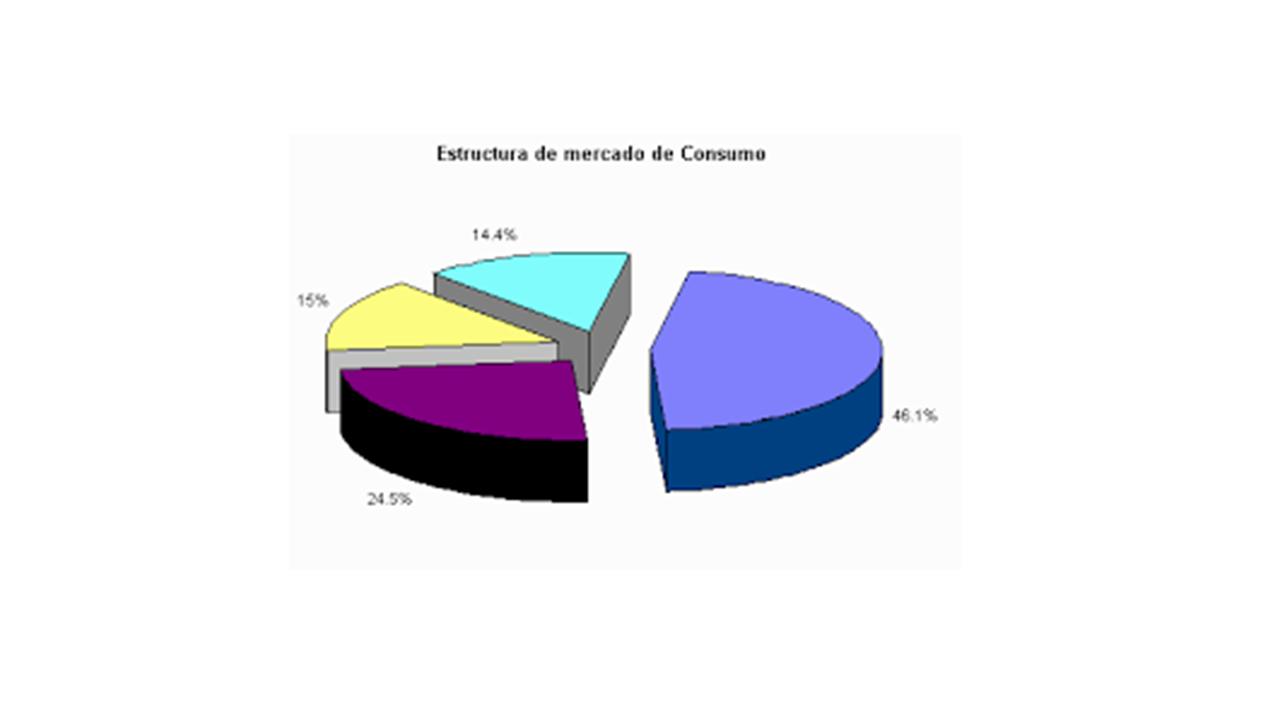
\includegraphics[width=.5\textwidth]{particion}
    & 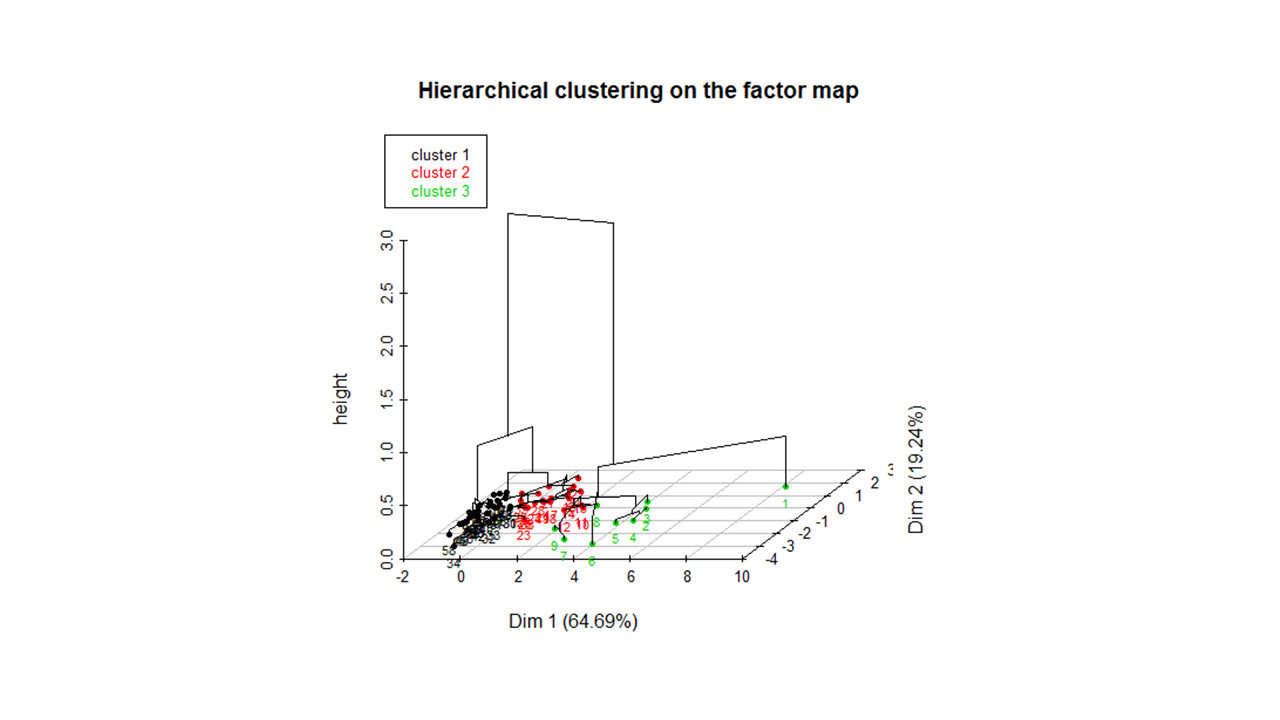
\includegraphics[width=.5\textwidth]{dendro1} \\
    \end{tabular}%
  %
  \caption{Particiones y Jerarquías}\label{klasificaciones}
\end{figure}
\end{frame}

\begin{frame}{Construcción de los grupos}
\LARGE Agrupación por particiones (K-medias)
\end{frame}
% 
\section{Agrupación por particiones}
\begin{frame}{Particiones}
Los datos para éste método son tablas con observaciones de variables de naturaleza continua o cuantitativas, y también se pueden utilizar las coordenadas obtenidas por un $ACP$, $ACS$, $ACM$.


Este método consiste en dividir el conjunto de objetos que se van a agrupar en un numero de grupos prefijado de manera que (\cite{PEGNA}):
\begin{itemize}
\item Cada objeto pertenezca a uno y solo uno de los grupos.
\item Todo objeto quede en algún grupo
\item Cada grupo sea lo más homogéneo posible.
\item Los grupos se distingan entre si lo máximo posible.
\end{itemize}
\end{frame}
% 
\begin{frame}{Algoritmo $K$ medias}
* Seleccionar un numero prefijado $K$ de puntos o centros iniciales y conformar el mismo número de grupos asignando los objetos al grupo más cercano, 

* Calcular los centros o promedios de cada grupo formado y luego reasignar los objetos a los nuevos grupos de acuerdo con su cercanía al centro de cada nuevo grupo, hasta que se estabilice la asignación con respecto a algún criterio de homogeneidad (optimalidad). En forma de algoritmo el procedimiento es como sigue\footnote{Adaptado de https://www.thoughtco.com/k-means-clustering-1019648}:
\end{frame}
% 
\begin{frame}
\begin{enumerate}
	\item Seleccionar aleatoriamente (o con algún criterio apropiado) $K$ puntos como centros de los grupos iniciales.

\item Utilizar algún criterio de distancia para asignar cada objeto al grupo cuyo centro se encuentre más cercano .\label{KMeanpaso2}

\item Recalcular los centros de los grupos como los promedios de los objetos del grupo.\label{KMeanpaso3}

\item Repetir los pasos (\ref{KMeanpaso2}) y (\ref{KMeanpaso3}) hasta que algún \textbf{criterio de optimalidad}  (por ejemplo, mayor homogeneidad dentro de los grupos y mayor heterogeneidad entre grupos) indique que no es posible mejorar los grupos.

\item Si no es posible mejorar suficientemente el criterio de optimalidad, terminar el proceso.
\end{enumerate}

Los pasos 2. y 3. garantizan que los centros se vayan desplazando en la dirección deseada para que los grupos sean cada vez más homogéneos.
\end{frame}
% 
\begin{frame}{Criterio de homogeneidad de Ward (optimalidad) para el algoritmo de K-medias}
\LARGE Consiste básicamente en minimizar la varianza dentro de los grupos y maximizar la varianza entre grupos.
\end{frame}
% 
% \begin{frame}{Criterio de homogeneidad de Ward (optimalidad) para el algoritmo de K-medias}
% Consiste básicamente en minimizar la varianza dentro de los grupos y maximizar la varianza entre grupos.
% \end{frame}
% % 
% \begin{frame}
% Matriz de datos centrados $\widetilde{X}$ particionada en $K$ submatrices que corresponden al numero de grupos en que se van a particionar los objetos observados así:
% \begin{equation*}
% X = \left( \mathbf{x^{\prime}_1}^, \ldots, \mathbf{x^{\prime}_{_K}} \right) = \left[ \begin{array}{c}
% \mathbf{x_1}\\
% \mathbf{x_2}\\
% \vdots\\
% \mathbf{x_{_K}}\\
% \end{array} \right], \quad \text{donde} \quad \mathbf{x_{_k}}  = \left[ \begin{array}{c}
% x_{11,k} \cdots x_{1p,k}\\
% x_{21,k} \cdots x_{2p,k}\\
% \vdots \quad \cdots \quad  \vdots\\
% x_{n_k 1,k} \cdots    x_{n_k p,k}\\
% \end{array} \right], \quad 
% \end{equation*}
% $n=\sum_{k=1}^K n_{_K}$
% \end{frame}
% % 
% \begin{frame}
% Ahora se define  la $i$ ésima fila de la submatriz $\mathbf{x_{_k}}$ como el vector:
% $$
% \mathbf{x_{i,k}} = \left(x_{i1,k},\ldots,x_{ip,k}\right)^\prime = \left[ \begin{array}{c}
% x_{i1,k}\\
% x_{i2,k}\\
% \vdots\\
% x_{ip,k}\\
% \end{array} \right], \quad i=1,\ldots,n_{_k} .
% $$
% y sea $\mathbf{\bar{x}_k} =
% (\bar{x}_{1,k}, \ldots , \bar{x}_{p,k} )^\prime $ el vector de medias del grupo $k$.
% \end{frame}
% % 
% \begin{frame}
% Se define $W$ la matriz de sumas de cuadrados dentro de grupos por
% \begin{equation} \label{scdg1}
% W= \sum_{k=1}^K \sum_{i=1}^{n_k}(\mathbf{x_{i,k}}-\mathbf{\bar{x}_k)} (\mathbf{x_{i,k}}-\mathbf{\bar{x}_k})^\prime
% \end{equation}
% de manera que
% \[
% w_{j  j'} = \left\{ \sum_{k=1}^K \sum_{i=1}^ {n_{_K}} \left( x_{ij,k} - \bar{x}_{j,k} \right) \left( x_{ij',k} - \bar{x}_{j',k} \right) \right\}
% \]
% \end{frame}
% 
\begin{frame}{Criterio de homogeneidad de Ward (optimalidad) para el algoritmo de K-medias}
Se definen las sumas de cuadrados dentro de grupos (SCDG):
\begin{equation}\label{scdg2}
SCDG_j= \sum_{k=1}^K \sum_{i=1}^ {n_{_K}} \left( x_{ij,k} - \bar{x}_{j,k} \right)^2
\end{equation}

El criterio de Ward o criterio de la traza,  consiste en minimizar la SCDG:
$$
\text{min} \sum_{j=1}^p SCDG_j
$$

% $$
% \min \left\lbrace  traza(W) \right\rbrace = \min \sum_{j=1}^p \sum_{k=1}^K \sum_{i=1}^ {n_{_K}} \left( x_{ij,k} - \bar{x}_{j,k} \right)^2
% $$
\end{frame}
% 
\begin{frame}
\LARGE{Indicadores para calcular el numero de grupos para el $k$- means}
\end{frame}

\begin{frame}{Índice de Carlinski- Habasz}

Carlinski- Habasz
También llamado criterio de razón de varianzas \footnote{Se enuentra entre otros en el paquete  \textbf{fpc} de $R$ ``Flexible Procedures of Clustering''.}  que utiliza el índice:
\[
CH_K= \frac{SCEG/(K-1)}{SCDG/(n-K)}
= \frac{SCEG}{SCDG}\frac{n-K}{K-1} 
\]
donde
\[
SCEG = \sum_{k=1}^K \sum_{j=1}^{p} n_k(\bar{x}_{jk}-\bar{x}_j)^2
\]
\textbf{el número óptimo de grupos se obtiene maximizando $CH_K$ con respecto a $K$}
\end{frame}
%
\begin{frame}{Índice de Hartigan}
El criterio de Hartigan incluye un nuevo grupo si:
$$Hrt=\frac{SCDG(k)-SCDG(k+1)}{{SCDG(k+1)}/(n-k+1)}>10 $$
donde como las sumas de cuadrados involucradas generalmente no satisfacen los supuestos requeridos para que el cociente tenga distribución $F$ suele utilizarse el valor empírico $10$ propuesto por Hartigan.
\end{frame}
%
\begin{frame}{Algunas características del algoritmo $K-$ means}
El algoritmo de $K$-medias se conoce en el contexto del aprendizaje estadístico como un \textbf{algoritmo no supervisado} por utilizar solo características de la \textbf{estructura interna de los objetos a agrupar}, es decir por sus propiedades o características. \vskip2mm

\textbf{Ventaja:} Muy \textbf{rápido y secillo} de aplicar.\vskip2mm

\textbf{Ventaja:} \textbf{Se puede optimizar} por la búsqueda de grupos estables, algoritmo que consiste en construir muchas Agrupaciones e identificar como grupos estables aquellos formados por objetos que quedan siempre en los mismos grupos. Este algoritmo se utiliza también posteriormente para agrupaciones mixtas.

\end{frame}
%
\begin{frame}
\textbf{Desventaja:} El hecho de que los centros móviles para la primera etapa sean elegidos de manera arbitraria hace que las agrupaciones sean dependientes de éstos y a su vez hace \textbf{inestable} el método. \vskip2mm

\textbf{Desventaja:} Como el número de grupos es prefijado, la agrupación puede conducir a \textbf{grupos difíciles de tipificar}, por ejemplo, si se va a agrupar un grupo de huesos de dos clases mamíferos como perros y lobos por la especie y se escoge $K>2$ los resultados muy seguramente son inconsistentes.

\textbf{Desventaja:} No es robusto cuando hay observaciones atípicas
\end{frame}
%
\begin{frame}
\LARGE {Ejemplo: Indicadores del Sistema Universitario Estatal (SUE)}

Que contiene datos de alrededor de 32 indicadores de educación superior para las 32 universidades estatales entre 2003 y 2012
\end{frame}
% 
\begin{frame}{Ejemplo}
{Agrupación de universidades del Sistema Universitario Estatal (SUE)}
Se utilizan seis de los 32 indicadores del SUE


Docentes de tiempo completo o equivalente (DCTC2012)

Gastos en personal administrativo  (GPA2012)

Matrícula de pregrado (MPRE2012)

Matrícula de posgrado (MPOS2012)

Graduados de pregrado (GrPre2012)

Graduados de posgrado (GrPos2012).
\end{frame}
%
\begin{frame}[fragile]
\frametitle{Agrupación de universidades DEL Sistema Universitario Estatal (SUE)}
\begin{block}{Algunos indicadores del SUE}
\begin{table}[!h]
\centering
\caption{\label{tab:sue}Primeras seis filas de indicadores del SUE}
\centering
\resizebox{\ifdim\width>\linewidth\linewidth\else\width\fi}{!}{
\begin{tabular}[t]{lrrrrrr}
\toprule
Universidades & DCTC2012 & GPA2012 & MPRE2012 & MPOS2012 & GrPre2012 & GrPos2012\\
\midrule
\cellcolor{gray!10}{NACIONAL} & \cellcolor{gray!10}{2161} & \cellcolor{gray!10}{347233353} & \cellcolor{gray!10}{42120} & \cellcolor{gray!10}{9299} & \cellcolor{gray!10}{4903} & \cellcolor{gray!10}{3181}\\
PEDAGOGICA & 440 & 7986738 & 9321 & 1614 & 1186 & 362\\
\cellcolor{gray!10}{UPTC} & \cellcolor{gray!10}{828} & \cellcolor{gray!10}{20641880} & \cellcolor{gray!10}{24644} & \cellcolor{gray!10}{2360} & \cellcolor{gray!10}{3190} & \cellcolor{gray!10}{1225}\\
CAUCA & 550 & 28539431 & 12859 & 700 & 1372 & 303\\
\cellcolor{gray!10}{TEC DE PEREIRA} & \cellcolor{gray!10}{442} & \cellcolor{gray!10}{15343348} & \cellcolor{gray!10}{15423} & \cellcolor{gray!10}{1319} & \cellcolor{gray!10}{1532} & \cellcolor{gray!10}{299}\\
\addlinespace
CALDAS & 418 & 12877924 & 12261 & 971 & 1953 & 266\\
\bottomrule
\end{tabular}}
\end{table}\end{block}
\end{frame}
%
\begin{frame}[fragile]
{Cálculo del indicador de Calinski-Harabasz para decidir el numero de grupos}
% \begin{block}{R Code}
\begin{table}[!h]
\centering
\caption{\label{tab:caHabas}Valores del índice de Carlinski-Habasz}
\centering
\resizebox{\ifdim\width>\linewidth\linewidth\else\width\fi}{!}{
\begin{tabular}[t]{lrrrrrrrrr}
\toprule
  & 2 & 3 & 4 & 5 & 6 & 7 & 8 & 9 & 10\\
\midrule
\cellcolor{gray!10}{res.sue\$All.index} & \cellcolor{gray!10}{371.8109} & \cellcolor{gray!10}{1098.372} & \cellcolor{gray!10}{1332.701} & \cellcolor{gray!10}{1304.734} & \cellcolor{gray!10}{1124.575} & \cellcolor{gray!10}{945.2354} & \cellcolor{gray!10}{790.8089} & \cellcolor{gray!10}{2852.949} & \cellcolor{gray!10}{3474.023}\\
\bottomrule
\end{tabular}}
\end{table}\[
CH_K= \frac{SCEG/(K-1)}{SCDG/(n-K)}
= \frac{SCEG}{SCDG}\frac{(n-K)}{(K-1)}
\]
% \end{block}
\end{frame}
%
\begin{frame}[fragile]
{Cálculo del indicador de Calinski-Harabasz para decidir el numero de grupos}
\setkeys{Gin}{width=1\textwidth, height=0.8\textheight,keepaspectratio} % para redefinir el tama?o de los graficos
\begin{figure}[H]
	\centering
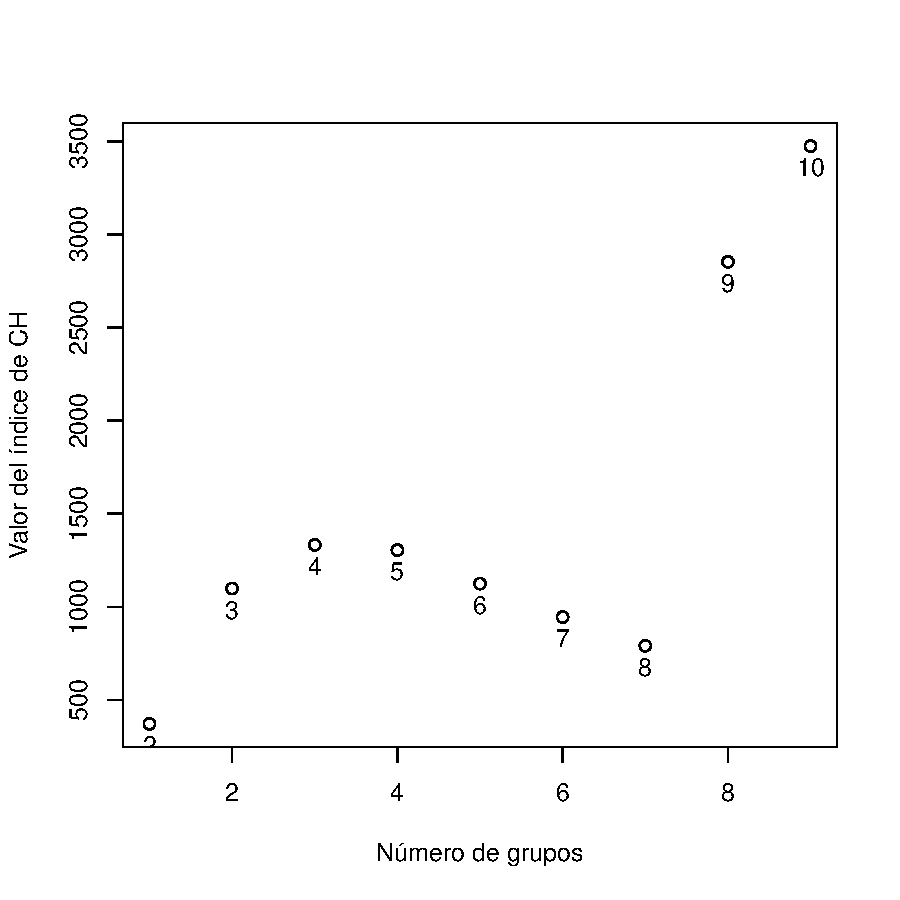
\includegraphics{8_Agrupaciones-015}
	\caption{Valores del índice de Carlinski - Habasz}\label{fig:CaHabasz}
\end{figure}
\end{frame}
%
\begin{frame}[fragile]
\scriptsize 
\begin{block}{Grupos por el C-H}
\begin{table}[!h]
\centering
\caption{\label{tab:gruposCaHabas}Grupos sugeridos por el índice de CH}
\centering
\resizebox{\ifdim\width>\linewidth\linewidth\else\width\fi}{!}{
\begin{tabular}[t]{lrlr}
\toprule
Universidad & grupo & Universidad & grupo\\
\midrule
\cellcolor{gray!10}{POPU DEL CESAR} & \cellcolor{gray!10}{1} & \cellcolor{gray!10}{CALDAS} & \cellcolor{gray!10}{6}\\
PACIFICO & 1 & LLANOS & 6\\
\cellcolor{gray!10}{UFPS\_OCANA} & \cellcolor{gray!10}{1} & \cellcolor{gray!10}{ATLANTICO} & \cellcolor{gray!10}{6}\\
MAGDALENA & 1 & QUINDIO & 6\\
\cellcolor{gray!10}{SUCRE} & \cellcolor{gray!10}{1} & \cellcolor{gray!10}{CUNDINAMARCA} & \cellcolor{gray!10}{6}\\
\addlinespace
CAUCA & 2 & UPTC & 7\\
\cellcolor{gray!10}{TEC DE PEREIRA} & \cellcolor{gray!10}{3} & \cellcolor{gray!10}{TEC DEL CHOCO} & \cellcolor{gray!10}{7}\\
CORDOBA & 3 & TOLIMA & 7\\
\cellcolor{gray!10}{DISTRITAL} & \cellcolor{gray!10}{3} & \cellcolor{gray!10}{PEDAGOGICA} & \cellcolor{gray!10}{8}\\
UNAD & 3 & AMAZONIA & 8\\
\addlinespace
\cellcolor{gray!10}{NACIONAL} & \cellcolor{gray!10}{4} & \cellcolor{gray!10}{MAY DE CNAMARCA} & \cellcolor{gray!10}{8}\\
SURCOLOMBIANA & 5 & UFPS\_CUCUTA & 8\\
\cellcolor{gray!10}{MILITAR} & \cellcolor{gray!10}{5} & \cellcolor{gray!10}{ANTIOQUIA} & \cellcolor{gray!10}{9}\\
NARINO & 5 & VALLE & 9\\
\cellcolor{gray!10}{PAMPLONA} & \cellcolor{gray!10}{5} & \cellcolor{gray!10}{UIS} & \cellcolor{gray!10}{10}\\
\addlinespace
GUAJIRA & 5 & CARTAGENA & 10\\
\bottomrule
\end{tabular}}
\end{table}\end{block}
\end{frame}
%
\begin{frame}[fragile]
{Tipificación de los grupos sugeridos por el índice de CH por los promedios de las varaibles:}
\tiny
\begin{block}{Descripción or los promedios de los grupos sugeridos por C-H}
\begin{table}[!h]
\centering
\caption{\label{tab:NediastipigrupCH}Promedios de las variables para los grupos sugeridos por el índice de CH}
\centering
\begin{tabular}[t]{lrrrrrrr}
\toprule
  & Group.1 & DCTC2012 & GPA2012 & MPRE2012 & MPOS2012 & GrPre2012 & GrPos2012\\
\midrule
\cellcolor{gray!10}{1} & \cellcolor{gray!10}{1} & \cellcolor{gray!10}{145.60} & \cellcolor{gray!10}{4328623} & \cellcolor{gray!10}{8950.00} & \cellcolor{gray!10}{147.20} & \cellcolor{gray!10}{1135.20} & \cellcolor{gray!10}{109.4}\\
8 & 8 & 282.25 & 7201681 & 10432.00 & 684.00 & 1263.25 & 244.0\\
\cellcolor{gray!10}{5} & \cellcolor{gray!10}{5} & \cellcolor{gray!10}{340.80} & \cellcolor{gray!10}{10007899} & \cellcolor{gray!10}{13133.00} & \cellcolor{gray!10}{851.20} & \cellcolor{gray!10}{1863.00} & \cellcolor{gray!10}{413.6}\\
6 & 6 & 347.20 & 12490477 & 12711.60 & 348.00 & 1456.00 & 153.8\\
\cellcolor{gray!10}{7} & \cellcolor{gray!10}{7} & \cellcolor{gray!10}{463.00} & \cellcolor{gray!10}{21754777} & \cellcolor{gray!10}{24130.67} & \cellcolor{gray!10}{1195.33} & \cellcolor{gray!10}{3075.00} & \cellcolor{gray!10}{617.0}\\
\addlinespace
10 & 10 & 533.50 & 47011123 & 19350.50 & 1365.00 & 1981.00 & 463.5\\
\cellcolor{gray!10}{2} & \cellcolor{gray!10}{2} & \cellcolor{gray!10}{550.00} & \cellcolor{gray!10}{28539431} & \cellcolor{gray!10}{12859.00} & \cellcolor{gray!10}{700.00} & \cellcolor{gray!10}{1372.00} & \cellcolor{gray!10}{303.0}\\
3 & 3 & 569.75 & 15856248 & 29838.75 & 1267.50 & 1855.25 & 276.5\\
\cellcolor{gray!10}{9} & \cellcolor{gray!10}{9} & \cellcolor{gray!10}{1391.50} & \cellcolor{gray!10}{66413127} & \cellcolor{gray!10}{31516.50} & \cellcolor{gray!10}{2999.00} & \cellcolor{gray!10}{3323.00} & \cellcolor{gray!10}{807.5}\\
4 & 4 & 2161.00 & 347233353 & 42120.00 & 9299.00 & 4903.00 & 3181.0\\
\bottomrule
\end{tabular}
\end{table}\end{block}
El grupo 1 tiene los menores promedios en todos los indicadores. Además, el grupo 1 junto con los grupos 8, 5, y 6 también tienen los menores promedios tanto en Docentes de tiempo completo (DCTC2012) como en Gastos de personal administrativo (GPA2012).
\end{frame}
%
\begin{frame}[fragile]

\tiny
\begin{block}{Grados de homogeneidad de los grupos sugeridos por el C-H}
\begin{table}[!h]
\centering
\caption{\label{tab:desvSttipigrupCH}Desviación estándar de los grupos sugeridos por el índice de CH}
\centering
\begin{tabular}[t]{lrrrrrrr}
\toprule
  & Group.1 & DCTC2012 & GPA2012 & MPRE2012 & MPOS2012 & GrPre2012 & GrPos2012\\
\midrule
\cellcolor{gray!10}{6} & \cellcolor{gray!10}{6} & \cellcolor{gray!10}{95.49} & \cellcolor{gray!10}{762449.8} & \cellcolor{gray!10}{5533.96} & \cellcolor{gray!10}{355.21} & \cellcolor{gray!10}{593.74} & \cellcolor{gray!10}{79.13}\\
1 & 1 & 103.59 & 702042.7 & 7483.67 & 262.22 & 1154.06 & 146.90\\
\cellcolor{gray!10}{8} & \cellcolor{gray!10}{8} & \cellcolor{gray!10}{112.98} & \cellcolor{gray!10}{809507.4} & \cellcolor{gray!10}{6956.78} & \cellcolor{gray!10}{634.31} & \cellcolor{gray!10}{700.24} & \cellcolor{gray!10}{82.46}\\
5 & 5 & 116.16 & 758930.3 & 6270.40 & 1026.74 & 1942.13 & 466.52\\
\cellcolor{gray!10}{10} & \cellcolor{gray!10}{10} & \cellcolor{gray!10}{139.30} & \cellcolor{gray!10}{3018201.1} & \cellcolor{gray!10}{772.87} & \cellcolor{gray!10}{712.76} & \cellcolor{gray!10}{1053.59} & \cellcolor{gray!10}{202.94}\\
\addlinespace
3 & 3 & 213.24 & 1143153.2 & 24048.97 & 618.54 & 915.35 & 297.47\\
\cellcolor{gray!10}{7} & \cellcolor{gray!10}{7} & \cellcolor{gray!10}{318.68} & \cellcolor{gray!10}{1386434.1} & \cellcolor{gray!10}{13213.48} & \cellcolor{gray!10}{1158.55} & \cellcolor{gray!10}{1484.84} & \cellcolor{gray!10}{589.02}\\
9 & 9 & 645.59 & 7383788.6 & 7455.03 & 338.00 & 161.22 & 10.61\\
\cellcolor{gray!10}{2} & \cellcolor{gray!10}{2} & \cellcolor{gray!10}{NA} & \cellcolor{gray!10}{NA} & \cellcolor{gray!10}{NA} & \cellcolor{gray!10}{NA} & \cellcolor{gray!10}{NA} & \cellcolor{gray!10}{NA}\\
4 & 4 & NA & NA & NA & NA & NA & NA\\
\bottomrule
\end{tabular}
\end{table}\end{block}
\end{frame}
%
\begin{frame}
A manera de conclusión, el hecho de que el índice de Carlinski - Habasz sugiera 10 grupos en un conjunto de 32 universidades, no parece muy eficiente. \vskip1mm 

No obstante, éste índice muestra un segundo valor alto (mínimo local) en 4 grupos como se observa en la Tabla tabla \ref{tab:caHabas}, lo cual podría sugerir solo 4 grupos, pero este agrupamiento no sería el sugerido estrictamente por el criterio $CH_K$.
\end{frame}
%
\begin{frame}[fragile]
{Ejemplo: Construcción de grupos por el índice de Hartigan}
En este ejemplo se muestra cómo pueden variar los agrupamientos dependiendo del índice que se utilice para seleccionar el numero de grupos. Ahora se van a construir los grupos de universidades del SUE, pero utilizando el índice de Hartigan.
%  del ejemplo \ref{anterior}
\begin{Schunk}
\begin{Sinput}
> res.sue.hart<-NbClust(xsue, distance = "euclidean", 
+                       min.nc = 2, max.nc = 10,
+                  method = "kmeans", index = "hartigan")
> # names(res.sue.hart) # contenido del archivo de salida res.sue.hart
> 
\end{Sinput}
\end{Schunk}
\end{frame}
%
\begin{frame}[fragile]
\tiny
\begin{block}{Índice de Hartigan}
\begin{table}[!h]
\centering
\caption{\label{tab:hartIndex}Valores del índice de Hartigan por número de grupos}
\centering
\begin{tabular}[t]{rrrrrrrrr}
\toprule
2 & 3 & 4 & 5 & 6 & 7 & 8 & 9 & 10\\
\midrule
\cellcolor{gray!10}{141.9087} & \cellcolor{gray!10}{25.331} & \cellcolor{gray!10}{9.8347} & \cellcolor{gray!10}{3.1921} & \cellcolor{gray!10}{1.2675} & \cellcolor{gray!10}{0.4165} & \cellcolor{gray!10}{78.9124} & \cellcolor{gray!10}{9.93} & \cellcolor{gray!10}{0.7751}\\
\bottomrule
\end{tabular}
\end{table}\begin{table}[!h]
\centering
\caption{\label{tab:hartgrups}Número de grupos sugerido por el índice de Hartigan paso de 2 a 3}
\centering
\begin{tabular}[t]{rr}
\toprule
Number\_clusters & Value\_Index\\
\midrule
\cellcolor{gray!10}{3} & \cellcolor{gray!10}{116.5777}\\
\bottomrule
\end{tabular}
\end{table}
\end{block}
\end{frame}
%
\begin{frame}[fragile]
\setkeys{Gin}{width=0.9\textwidth, height=0.9\textheight,keepaspectratio} % para redefinir el tama?o de los graficos
\begin{figure}[H]
	\centering
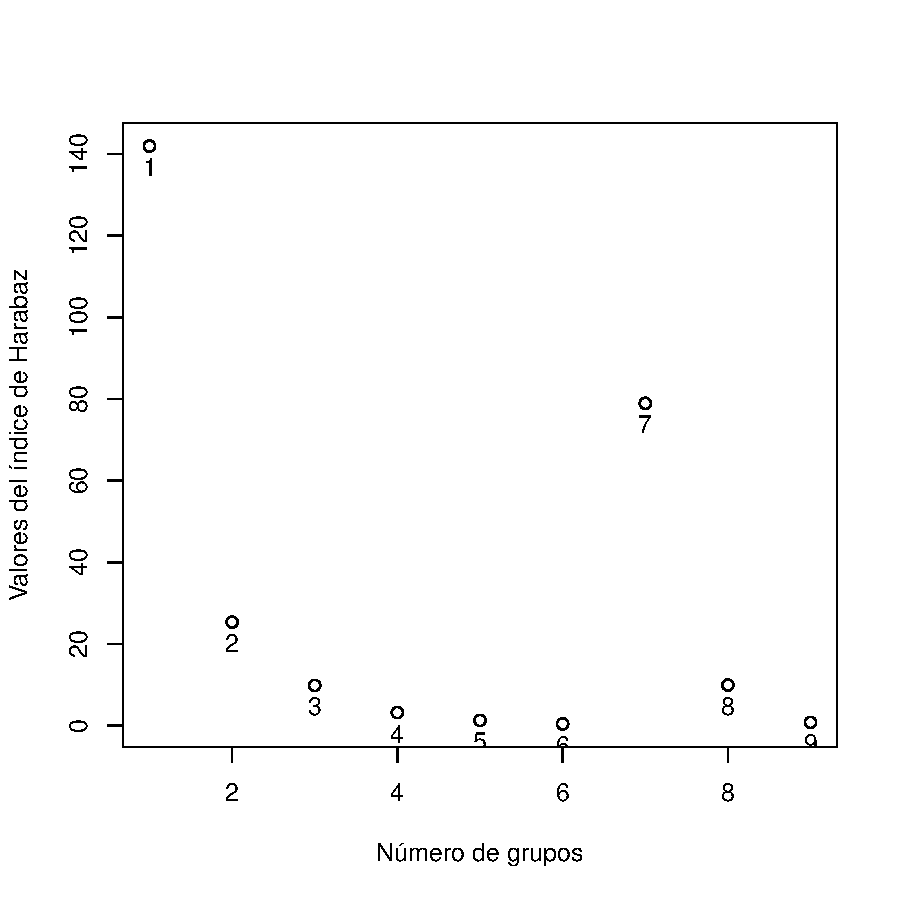
\includegraphics{8_Agrupaciones-021}
	\caption{Valores del índice de Hartigan}\label{fig:Hartigan}
\end{figure}
\end{frame}
% 
\begin{frame}
\tiny
\begin{block}{Miembros de los grupos sugeridos por el índice de Hartigan}
\begin{table}[!h]
\centering
\caption{\label{tab:hartgrupsugeridos}Grupos sugeridos por el índice de Hartigan}
\centering
\begin{tabular}[t]{lrlr}
\toprule
Universidades & Grupos & Universidades & Grupos\\
\midrule
\cellcolor{gray!10}{PEDAGOGICA} & \cellcolor{gray!10}{1} & \cellcolor{gray!10}{TOLIMA} & \cellcolor{gray!10}{1}\\
UPTC & 1 & QUINDIO & 1\\
\cellcolor{gray!10}{CAUCA} & \cellcolor{gray!10}{1} & \cellcolor{gray!10}{UFPS\_CUCUTA} & \cellcolor{gray!10}{1}\\
TEC DE PEREIRA & 1 & UFPS\_OCANA & 1\\
\cellcolor{gray!10}{CALDAS} & \cellcolor{gray!10}{1} & \cellcolor{gray!10}{PAMPLONA} & \cellcolor{gray!10}{1}\\
\addlinespace
CORDOBA & 1 & MAGDALENA & 1\\
\cellcolor{gray!10}{SURCOLOMBIANA} & \cellcolor{gray!10}{1} & \cellcolor{gray!10}{CUNDINAMARCA} & \cellcolor{gray!10}{1}\\
AMAZONIA & 1 & SUCRE & 1\\
\cellcolor{gray!10}{MILITAR} & \cellcolor{gray!10}{1} & \cellcolor{gray!10}{GUAJIRA} & \cellcolor{gray!10}{1}\\
TEC DEL CHOCO & 1 & DISTRITAL & 1\\
\addlinespace
\cellcolor{gray!10}{LLANOS} & \cellcolor{gray!10}{1} & \cellcolor{gray!10}{UNAD} & \cellcolor{gray!10}{1}\\
POPU DEL CESAR & 1 & NACIONAL & 2\\
\cellcolor{gray!10}{MAY DE CNAMARCA} & \cellcolor{gray!10}{1} & \cellcolor{gray!10}{ANTIOQUIA} & \cellcolor{gray!10}{3}\\
PACIFICO & 1 & VALLE & 3\\
\cellcolor{gray!10}{ATLANTICO} & \cellcolor{gray!10}{1} & \cellcolor{gray!10}{UIS} & \cellcolor{gray!10}{3}\\
\addlinespace
NARINO & 1 & CARTAGENA & 3\\
\bottomrule
\end{tabular}
\end{table}\end{block}
\end{frame}
%
\begin{frame}[fragile]
% {Tipificación por los promedios de las variables de los grupos sugeridos el índice de Hartigan:}
\tiny
\begin{block}{Promedios por grupos}
\begin{table}[!h]
\centering
\caption{\label{tab:mediashartgrupsugeridos}Promedios de las varaiables para los grupos sugeridos por el índice de Hartigan}
\centering
\begin{tabular}[t]{rrrrrrr}
\toprule
Group.1 & DCTC2012 & GPA2012 & MPRE2012 & MPOS2012 & GrPre2012 & GrPos2012\\
\midrule
\cellcolor{gray!10}{1} & \cellcolor{gray!10}{352.41} & \cellcolor{gray!10}{11858166} & \cellcolor{gray!10}{15566.93} & \cellcolor{gray!10}{697.19} & \cellcolor{gray!10}{1679.33} & \cellcolor{gray!10}{282.22}\\
2 & 2161.00 & 347233353 & 42120.00 & 9299.00 & 4903.00 & 3181.00\\
\cellcolor{gray!10}{3} & \cellcolor{gray!10}{962.50} & \cellcolor{gray!10}{56712125} & \cellcolor{gray!10}{25433.50} & \cellcolor{gray!10}{2182.00} & \cellcolor{gray!10}{2652.00} & \cellcolor{gray!10}{635.50}\\
\bottomrule
\end{tabular}
\end{table}\end{block}
\end{frame}
%
\begin{frame}[fragile]
\tiny
\begin{block}{Desviaciones estándar por grupos}
\begin{table}[!h]
\centering
\caption{\label{tab:mediashartgrupsugeridos}Desviaciones estándar de las varaiables para los grupos sugeridos por el índice de Hartigan}
\centering
\begin{tabular}[t]{rrrrrrr}
\toprule
Group.1 & DCTC2012 & GPA2012 & MPRE2012 & MPOS2012 & GrPre2012 & GrPos2012\\
\midrule
\cellcolor{gray!10}{1} & \cellcolor{gray!10}{197.12} & \cellcolor{gray!10}{6329666} & \cellcolor{gray!10}{12664.44} & \cellcolor{gray!10}{742.21} & \cellcolor{gray!10}{1222.73} & \cellcolor{gray!10}{317.59}\\
2 & NA & NA & NA & NA & NA & NA\\
\cellcolor{gray!10}{3} & \cellcolor{gray!10}{625.13} & \cellcolor{gray!10}{12111532} & \cellcolor{gray!10}{8249.98} & \cellcolor{gray!10}{1047.57} & \cellcolor{gray!10}{989.45} & \cellcolor{gray!10}{230.68}\\
\bottomrule
\end{tabular}
\end{table}\end{block}
\end{frame}
%
\begin{frame}{Ejemplo: Comparación de las clasificaciones sigeridas por los índices de Carlinski-Harabas y Hartigan.}
La otra clasificación sugerida por el índice de Hartigan, aunque no es la que este índice sugiere estrictamente por no ser el número de grupos donde aparece el primer máximo, es en 8 grupos y se muestran en la Tabla \ref{tab:hartgrupsugeridos_8}. 

\end{frame}

\begin{frame}
\tiny
\begin{table}[!h]
\centering
\caption{\label{tab:hartgrupsugeridos_8}Ocho grupos sugeridos por el máximo local del índice de Hartigan}
\centering
\begin{tabular}[t]{lrlr}
\toprule
Universidades & Grupos & Universidades & Grupos\\
\midrule
\cellcolor{gray!10}{POPU DEL CESAR} & \cellcolor{gray!10}{1} & \cellcolor{gray!10}{NARINO} & \cellcolor{gray!10}{5}\\
PACIFICO & 1 & PAMPLONA & 5\\
\cellcolor{gray!10}{UFPS\_OCANA} & \cellcolor{gray!10}{1} & \cellcolor{gray!10}{GUAJIRA} & \cellcolor{gray!10}{5}\\
MAGDALENA & 1 & CALDAS & 6\\
\cellcolor{gray!10}{SUCRE} & \cellcolor{gray!10}{1} & \cellcolor{gray!10}{LLANOS} & \cellcolor{gray!10}{6}\\
\addlinespace
ANTIOQUIA & 2 & ATLANTICO & 6\\
\cellcolor{gray!10}{VALLE} & \cellcolor{gray!10}{2} & \cellcolor{gray!10}{QUINDIO} & \cellcolor{gray!10}{6}\\
UIS & 2 & CUNDINAMARCA & 6\\
\cellcolor{gray!10}{CARTAGENA} & \cellcolor{gray!10}{2} & \cellcolor{gray!10}{UPTC} & \cellcolor{gray!10}{7}\\
TEC DE PEREIRA & 3 & CAUCA & 7\\
\addlinespace
\cellcolor{gray!10}{CORDOBA} & \cellcolor{gray!10}{3} & \cellcolor{gray!10}{TEC DEL CHOCO} & \cellcolor{gray!10}{7}\\
DISTRITAL & 3 & TOLIMA & 7\\
\cellcolor{gray!10}{UNAD} & \cellcolor{gray!10}{3} & \cellcolor{gray!10}{PEDAGOGICA} & \cellcolor{gray!10}{8}\\
NACIONAL & 4 & AMAZONIA & 8\\
\cellcolor{gray!10}{SURCOLOMBIANA} & \cellcolor{gray!10}{5} & \cellcolor{gray!10}{MAY DE CNAMARCA} & \cellcolor{gray!10}{8}\\
\addlinespace
MILITAR & 5 & UFPS\_CUCUTA & 8\\
\bottomrule
\end{tabular}
\end{table}\end{frame}
%
\begin{frame}
\tiny
\begin{table}[!h]
\centering
\caption{\label{tab:comparación_grupos}Comparación de grupos sugridos por CH y Hartigan}
\centering
\resizebox{\ifdim\width>\linewidth\linewidth\else\width\fi}{!}{
\begin{tabular}[t]{llrrlrr}
\toprule
  & Universidad\_1 & Grupos C-H\_1 & Grupos Hrti\_1 & Universidad\_2 & Grupos C-H\_2 & Grupos Hrti\_2\\
\midrule
\cellcolor{gray!10}{12} & \cellcolor{gray!10}{MAGDALENA} & \cellcolor{gray!10}{1} & \cellcolor{gray!10}{1} & \cellcolor{gray!10}{ATLANTICO} & \cellcolor{gray!10}{6} & \cellcolor{gray!10}{6}\\
17 & PACIFICO & 1 & 1 & CALDAS & 6 & 6\\
\cellcolor{gray!10}{20} & \cellcolor{gray!10}{POPU DEL CESAR} & \cellcolor{gray!10}{1} & \cellcolor{gray!10}{1} & \cellcolor{gray!10}{CUNDINAMARCA} & \cellcolor{gray!10}{6} & \cellcolor{gray!10}{6}\\
22 & SUCRE & 1 & 1 & LLANOS & 6 & 6\\
\cellcolor{gray!10}{28} & \cellcolor{gray!10}{UFPS\_OCANA} & \cellcolor{gray!10}{1} & \cellcolor{gray!10}{1} & \cellcolor{gray!10}{QUINDIO} & \cellcolor{gray!10}{6} & \cellcolor{gray!10}{6}\\
\addlinespace
6 & CAUCA & 2 & 7 & TEC DEL CHOCO & 7 & 7\\
\cellcolor{gray!10}{7} & \cellcolor{gray!10}{CORDOBA} & \cellcolor{gray!10}{3} & \cellcolor{gray!10}{3} & \cellcolor{gray!10}{TOLIMA} & \cellcolor{gray!10}{7} & \cellcolor{gray!10}{7}\\
9 & DISTRITAL & 3 & 3 & UPTC & 7 & 7\\
\cellcolor{gray!10}{24} & \cellcolor{gray!10}{TEC DE PEREIRA} & \cellcolor{gray!10}{3} & \cellcolor{gray!10}{3} & \cellcolor{gray!10}{AMAZONIA} & \cellcolor{gray!10}{8} & \cellcolor{gray!10}{8}\\
30 & UNAD & 3 & 3 & MAY DE CNAMARCA & 8 & 8\\
\addlinespace
\cellcolor{gray!10}{15} & \cellcolor{gray!10}{NACIONAL} & \cellcolor{gray!10}{4} & \cellcolor{gray!10}{4} & \cellcolor{gray!10}{PEDAGOGICA} & \cellcolor{gray!10}{8} & \cellcolor{gray!10}{8}\\
10 & GUAJIRA & 5 & 5 & UFPS\_CUCUTA & 8 & 8\\
\cellcolor{gray!10}{14} & \cellcolor{gray!10}{MILITAR} & \cellcolor{gray!10}{5} & \cellcolor{gray!10}{5} & \cellcolor{gray!10}{ANTIOQUIA} & \cellcolor{gray!10}{9} & \cellcolor{gray!10}{2}\\
16 & NARINO & 5 & 5 & VALLE & 9 & 2\\
\cellcolor{gray!10}{18} & \cellcolor{gray!10}{PAMPLONA} & \cellcolor{gray!10}{5} & \cellcolor{gray!10}{5} & \cellcolor{gray!10}{CARTAGENA} & \cellcolor{gray!10}{10} & \cellcolor{gray!10}{2}\\
\addlinespace
23 & SURCOLOMBIANA & 5 & 5 & UIS & 10 & 2\\
\bottomrule
\end{tabular}}
\end{table}\end{frame}


\section{Agrupaciones jerárquicas}
\begin{frame}{Agrupaciones jerárquicas}
Categorías taxonómicas principales definidas en el Sistema de Información de la Naturaleza: Reino, Filo, Clase, Orden, Familia, Género, Especie.
\begin{figure}[H]
\centering
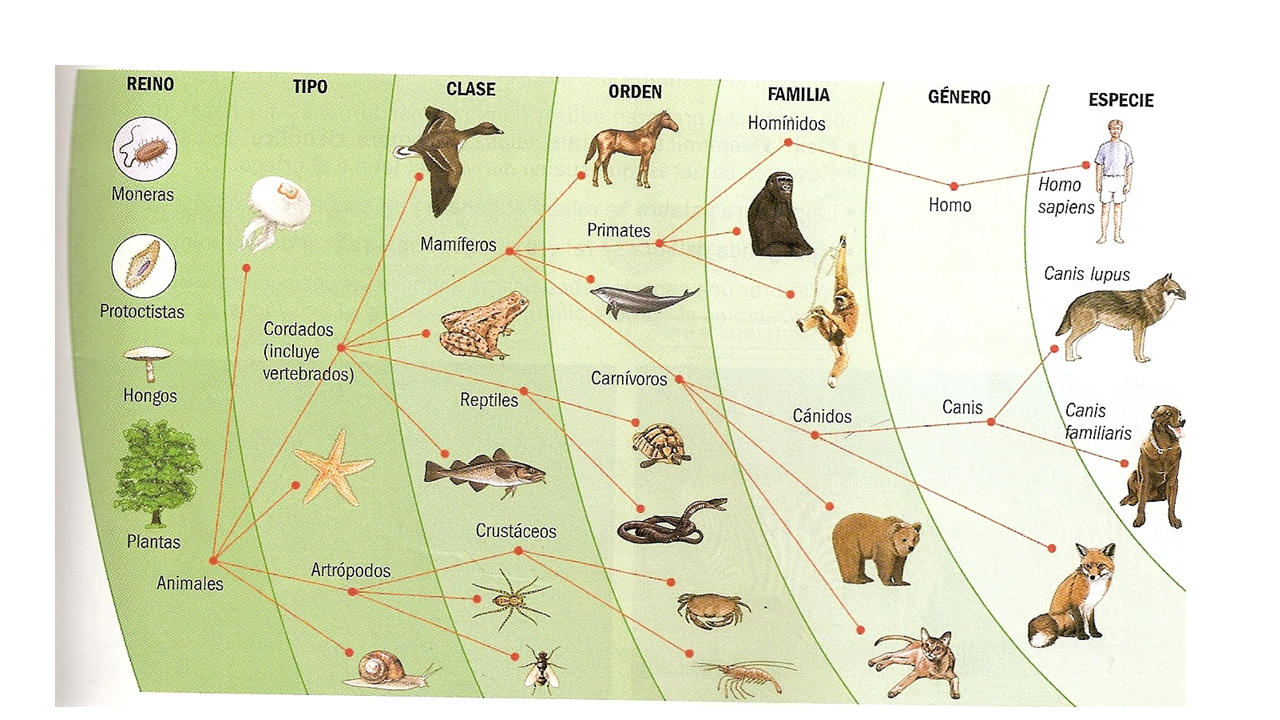
\includegraphics[width=.8\textwidth]{jerarquias1}
\caption{Categorías taxonómicas}\label{fig:agrjerarquicas1}
\end{figure}
\end{frame}
%
\begin{frame}{Agrupaciones jerárquicas}
Consiste construir grupos por aglomeración (ascendente)\vskip1mm
o por división (descendente) hasta conseguir grupos de objetos tan similares como sea posible dentro de los grupos.
\begin{figure}[H]
\centering
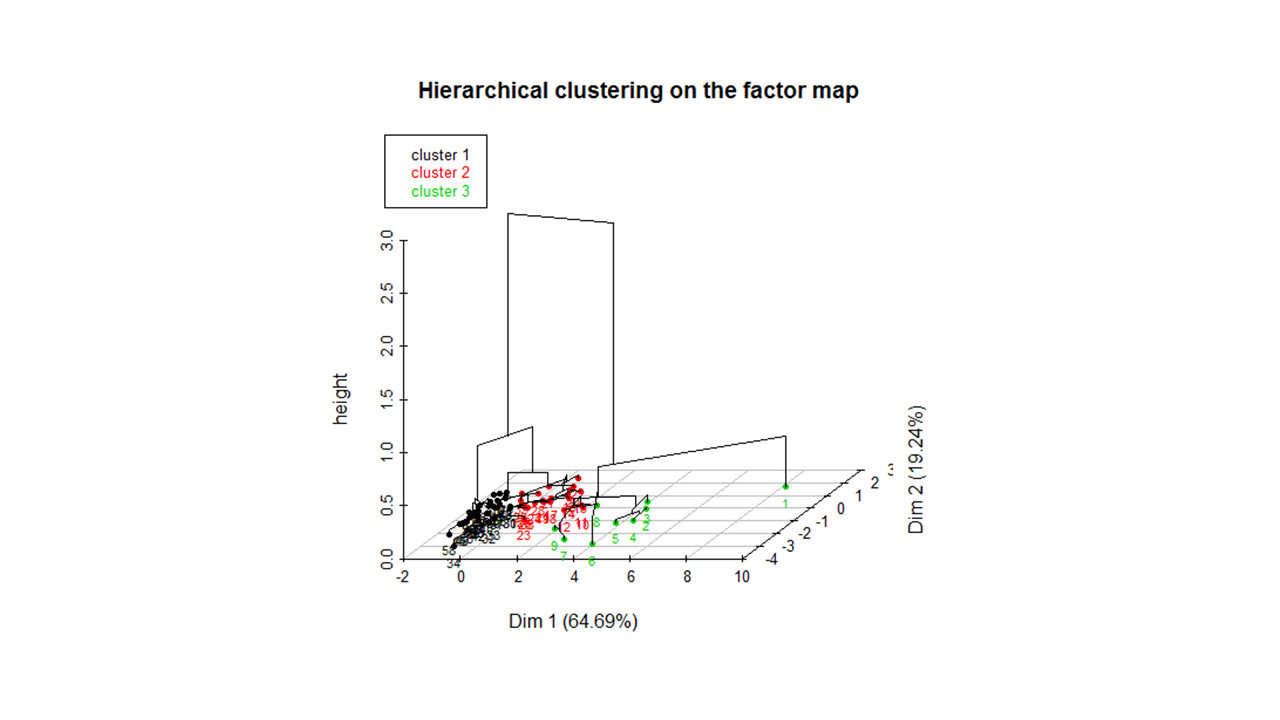
\includegraphics[width=.8\textwidth]{jerarquias2}
\caption{Agrupamiento por jerarqías}\label{fig:agrjerarquicas2}
\end{figure}
\end{frame}
%
\begin{frame}
{Divisiones}
División descendente del total a subgrupos hacia los objetos
División ascendenter de los objetos al total
\end{frame}
%
\begin{frame} {Algoritmo para el método de aglomeración ascendente}
\begin{enumerate}
\item Comenzar con tantos grupos como objetos, $ G=n $, de manera que las distancias entre grupos en este paso son las distancias entre los objetos originales.
\item Identificar los dos objetos  cercanos y formar con ellos un grupo.\label{seleccionar}
\item Representar el nuevo grupo construido en (\ref{seleccionar}) por un nuevo objeto, por ejemplo por el promedio del grupo y buscar nuevamente el objeto  cercano a éste para construir un nuevo grupo. \label{sustituir}
\item Repetir (\ref{seleccionar})  y  (\ref{sustituir})  hasta que todos los objetos queden agrupados en un único grupo.
\end{enumerate}
\end{frame}
%
\begin{frame}{Criterios para definir distancias entre grupos: }
\scriptsize
$ A $ y $ B $ grupos con $ n_a $ y $ n_b $ objetos, 
$ (AB) $ fusión de $A$ y $B$ con $ n_a+n_b $ objetos. Entonces la distancia del nuevo grupo $ (AB) $, a otro grupo $ C $ con $ n_c $ objetos se define por alguno de los siguientes criterios:

\textbf{Vecino  cercano:}\\
\[ d(C;AB)=\min (d_{CA},d_{CB}) \]

\textbf{Vecino  lejano:}
\[ d(C;AB)=\max (d_{CA};d_{CB}) \]

\textbf{Media de grupos:}
\[ d(C;AB)=\frac{n_a}{n_a+n_b}d_{CA}+\frac{n_b}{n_a+n_b}d_{CB} \]

\textbf{Método del centroide:}
\[ d^2(C;AB)=\frac{n_a}{n_a+n_b}d^2_{CA}+\frac{n_b}{n_a+n_b}d^2_{CB}-\frac{n_a n_b}{(n_a+n_b)^2} d^2_{AB} \]


\end{frame}
%
\begin{frame}{Método de Ward:}
Sumas de cuadrados dentro de grupos (SCDG):
\begin{equation}\label{scdg2}
W = \sum_{k=1}^K \sum_{i=1}^ {n_{_K}} \left( x_{ij,k} - \bar{x}_{j,k} \right)^2
\end{equation}

\begin{enumerate}
\item Suponer que cada objeto forma un grupo de manera que $ K = n $ y por tanto $  W = 0 $.
\item Unir los objetos que tengan la menor distancia euclídea entre ellos de manera que la unión aumente lo mínimo posible el valor de $ W $. Entonces quedan $ n-1 $ grupos de un objeto y un grupo de dos objetos.
\item Calcular $W$ para la nueva agrupación y unir los grupos que tengan la menor distancia euclídea entre ellos de manera que la unión aumente lo mínimo posible el valor de $ W $.\label{ward3}
\item Repetir el paso (\ref{ward3}) hasta que se obtenga un solo grupo.
\end{enumerate}
\end{frame}
%
\begin{frame}
El algoritmo para construir los grupos con el método de Ward se puede representar gráficamente en un \textbf{Dendrograma} de la siguiente manera:

\begin{enumerate}
\item Ubicar los objetos iniciales en la parte inferior del gráfico.
\item Trazar líneas verticales entre objetos con alturas \textbf{proporcionales a las distancias} entre éstos y líneas horizontales que indiquen las uniones entre ellos.
\item Repetir $ (1) $ y $ (2) $ hasta que todos los objetos estén conectados.
\end{enumerate}
\end{frame}
%
\begin{frame}{Ejemplo}
En este ejemplo se utiliza nuevamente el archivo de indicadores del SUE del ejemplo  \ref{carlHabasz} para construir una  agrupación jerárquica  de universidades por aglomeriación con el método de ward y se compara con las dos obtenidas por el método K-means.
\end{frame}
%
\begin{frame}[fragile]
\end{frame}
%
\begin{frame}[fragile]
\begin{figure}
\centering
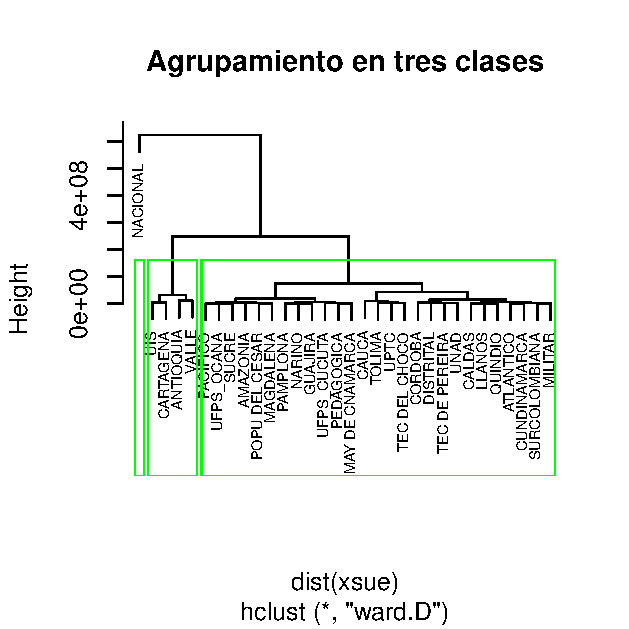
\includegraphics{8_Agrupaciones-clus1}
\caption{Agrupación jerárquica de universidades del SUE}\label{fig:dendroUnis}
\end{figure}

\end{frame}
%
\begin{frame}[fragile]
% \setkeys{Gin}{width=0.8\textwidth, height=0.5\textheight,keepaspectratio} % para redefinir el
\begin{figure}
\centering
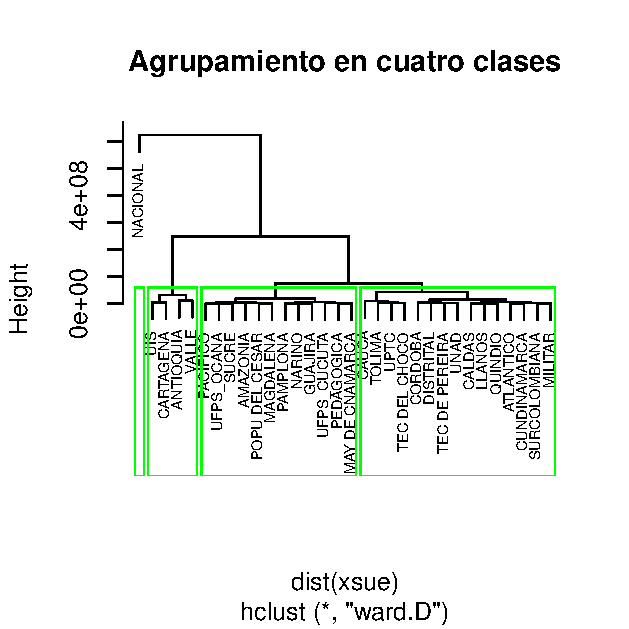
\includegraphics{8_Agrupaciones-031}
\caption{Agrupamiento jerárquico de univerisidades del SUE }\label{fig:dendroUnis4G}
\end{figure}
\end{frame}
%
\begin{frame}[fragile]
\begin{block}{Promedios de los grupos}
\begin{table}[!h]
\centering
\caption{\label{tab:mediasGr}Medias}
\centering
\resizebox{\ifdim\width>\linewidth\linewidth\else\width\fi}{!}{
\begin{tabular}[t]{lrrrrrrr}
\toprule
  & Group.1 & DCTC2012 & GPA2012 & MPRE2012 & MPOS2012 & GrPre2012 & GrPos2012\\
\midrule
\cellcolor{gray!10}{2} & \cellcolor{gray!10}{2} & \cellcolor{gray!10}{241.8333} & \cellcolor{gray!10}{6569468} & \cellcolor{gray!10}{10785.50} & \cellcolor{gray!10}{384.5833} & \cellcolor{gray!10}{1496.083} & \cellcolor{gray!10}{175.6667}\\
3 & 3 & 440.8667 & 16089124 & 19392.07 & 947.2667 & 1825.933 & 367.4667\\
\cellcolor{gray!10}{4} & \cellcolor{gray!10}{4} & \cellcolor{gray!10}{962.5000} & \cellcolor{gray!10}{56712125} & \cellcolor{gray!10}{25433.50} & \cellcolor{gray!10}{2182.0000} & \cellcolor{gray!10}{2652.000} & \cellcolor{gray!10}{635.5000}\\
1 & 1 & 2161.0000 & 347233353 & 42120.00 & 9299.0000 & 4903.000 & 3181.0000\\
\bottomrule
\end{tabular}}
\end{table}\end{block}
\end{frame}
%
\begin{frame}{Agrupaciones mixtas}
Utilización de una mezcla iterativa del método $K$-medias y el método de Agrupación jerárquica.

Algoritmo
\begin{itemize}
\item Hacer una partición inicial alrededor de centros móviles (k-means) para obtener unos cuantos grupos o incluso decenas de grupos homogéneos
\item Hacer una  partición jerárquica de estos grupos
\item Utilizar el Dendrograma para escoger la partición (o particiones) a realizar
\item Utilizar nuevamente los centros móviles para optimizar la partición escogida utilizando los grupos estables construidos a partir del k-means.
\end{itemize}
También se puede aplicar sobre los factores obtenidos por medio de $ACP$, $ACS$ o $ACM$, para producir agrupaciones más estables.
\end{frame}
%
\begin{frame}{Ejemplo ARWU por países}
\small
Indicadores:

Alumni: Número de egresados han recibido premios Nobel o medallas Field (Alumni y Award respectivamente), 

Award: Número de docentes o investigadores (D-I) activos que han recibido premios Nobel o medallas Field

HiCi: número de investigadores altamente citados seleccionadoos por el Thomson Reuters (), 

N.S: número de artículos publicados en las revistas Nature y Science (), 

PUB: número de artículos citados en el Science Citation Index () y 

PCP: rendimiento (producción de artículos por D-I) per cápita de una universidad (). 

El ranking agrupar alrededor de 1200 universidades de todo el mundo y publica los resultados de las primeras 500 anualmente desde 2003.
Para este ejemplo se calcularon los promedios de los indicadores de las 100 primeras universidades por país de la agrupación publicada por el ARWU en 2015.
\end{frame}
%
\begin{frame}[fragile]
\footnotesize
\begin{Schunk}
\begin{Soutput}
 [1] "Institution"   "Region"        "Country"       "Regional.Rank"
 [5] "World.Rank"    "National.Rank" "Alumni"        "Award"        
 [9] "HiCi"          "N.S"           "PUB"           "PCP"          
[13] "Total.Score"  
\end{Soutput}
\end{Schunk}
\end{frame}
%
\begin{frame}[fragile]
\scriptsize
\begin{block}{Promedios por país}
\begin{table}[!h]
\centering
\caption{\label{tab:arwuclus}Promedio de indicadores del ARWU por país}
\centering
\begin{tabular}[t]{lrrrrrr}
\toprule
  & Alumni & Award & HiCi & N.S & PUB & PCP\\
\midrule
\cellcolor{gray!10}{AS} & \cellcolor{gray!10}{17.30} & \cellcolor{gray!10}{8.90} & \cellcolor{gray!10}{26.40} & \cellcolor{gray!10}{21.63} & \cellcolor{gray!10}{56.10} & \cellcolor{gray!10}{27.73}\\
BE & 7.50 & 15.40 & 17.60 & 15.10 & 54.40 & 30.40\\
\cellcolor{gray!10}{CA} & \cellcolor{gray!10}{21.68} & \cellcolor{gray!10}{14.25} & \cellcolor{gray!10}{31.50} & \cellcolor{gray!10}{26.70} & \cellcolor{gray!10}{63.23} & \cellcolor{gray!10}{24.92}\\
DE & 19.60 & 21.50 & 16.60 & 24.75 & 52.40 & 28.85\\
\cellcolor{gray!10}{FI} & \cellcolor{gray!10}{16.00} & \cellcolor{gray!10}{17.80} & \cellcolor{gray!10}{22.80} & \cellcolor{gray!10}{20.60} & \cellcolor{gray!10}{52.70} & \cellcolor{gray!10}{28.20}\\
\addlinespace
FR & 39.10 & 31.30 & 16.63 & 22.77 & 45.90 & 34.07\\
\cellcolor{gray!10}{GE} & \cellcolor{gray!10}{27.48} & \cellcolor{gray!10}{22.62} & \cellcolor{gray!10}{17.48} & \cellcolor{gray!10}{21.86} & \cellcolor{gray!10}{46.96} & \cellcolor{gray!10}{27.42}\\
IR & 31.50 & 19.90 & 24.90 & 20.80 & 41.60 & 26.50\\
\cellcolor{gray!10}{JP} & \cellcolor{gray!10}{23.62} & \cellcolor{gray!10}{12.58} & \cellcolor{gray!10}{28.94} & \cellcolor{gray!10}{32.20} & \cellcolor{gray!10}{63.32} & \cellcolor{gray!10}{29.36}\\
NL & 23.70 & 18.15 & 27.90 & 25.15 & 48.00 & 29.25\\
\addlinespace
\cellcolor{gray!10}{NW} & \cellcolor{gray!10}{22.00} & \cellcolor{gray!10}{33.30} & \cellcolor{gray!10}{17.60} & \cellcolor{gray!10}{13.50} & \cellcolor{gray!10}{46.60} & \cellcolor{gray!10}{24.30}\\
RU & 46.80 & 34.10 & 0.00 & 9.60 & 52.40 & 31.20\\
\cellcolor{gray!10}{SE} & \cellcolor{gray!10}{24.37} & \cellcolor{gray!10}{29.60} & \cellcolor{gray!10}{20.63} & \cellcolor{gray!10}{20.27} & \cellcolor{gray!10}{45.63} & \cellcolor{gray!10}{29.63}\\
SW & 22.27 & 26.60 & 28.50 & 30.57 & 46.80 & 36.20\\
\cellcolor{gray!10}{UK} & \cellcolor{gray!10}{28.66} & \cellcolor{gray!10}{30.97} & \cellcolor{gray!10}{33.10} & \cellcolor{gray!10}{31.56} & \cellcolor{gray!10}{55.47} & \cellcolor{gray!10}{29.10}\\
\addlinespace
US & 25.66 & 29.61 & 44.42 & 37.37 & 55.43 & 30.79\\
\bottomrule
\end{tabular}
\end{table}\end{block}
\end{frame}
%
\begin{frame}[fragile]
\begin{figure}[H]
\centering
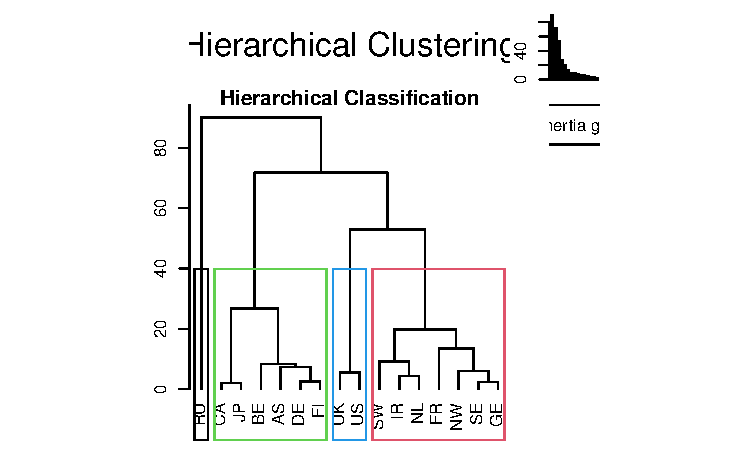
\includegraphics{8_Agrupaciones-035}
\caption{El dendrogaram sugiere cuatro grupos, uno de los cuales formado por un solo país}\label{fig:arwupaises4grup}
\end{figure}
\end{frame}
% % 
\begin{frame}{Indicadores para la descripción de los grupos}
\begin{itemize}
	\item \textbf{Mean in category:} Media de la variable en el grupo
	\item \textbf{Overall mean:} Promedio general de la variable
	\item \textbf{v.test:} Indicador de la diferencia entre la media del grupo y la media general. Entre mayor sea su valor mayor será la distancia entre la media del grupo y la media de todas las universidades.
	\item \textbf{sd in category:} Desviación estándar de la variable en el grupo
	\item \textbf{Overall sd:} Desviación estándar general
	\item \textbf{p.value:} Valor con el que se rechazaría la hipótesis de igualdad de media del grupo y media general.
\end{itemize}
\end{frame}
%
\begin{frame}{Valor test y valor p}
Éstas tablas también incluyen el valor test para la prueba de la hipótesis de que la media de la clase k ($\mu_k$) es igual a la media general ($\mu$) ($H_o: \mu_k = \mu$), el cual para la clase $k$ y la variable $X_j$ se define por: 
$$v.test = t_k = \frac{\bar{x}_{j,k} - \bar{x}}{s_{j,k}}$$
donde $\bar{x}_{j,k}$ es la media de $X_j$ en la clase $k$, $\bar{x}$ es la media general de todo el conjunto de datos y  
$${s_{j,k}} = \frac{n-n_k}{n-1}s^2(x_j)$$
La última columna de las tablas muestra el valor $p$ con el que se rechaza $H_o: \mu_k = \mu$
\end{frame}
%
\begin{frame}[fragile]
\end{frame}
%
\begin{frame}[fragile]
\begin{block}{Grupo1}
\begin{table}[!h]
\centering
\caption{\label{tab:arwuclus1}Indicadores para descripción del Grupo 1}
\centering
\resizebox{\ifdim\width>\linewidth\linewidth\else\width\fi}{!}{
\begin{tabular}[t]{lrrrrrr}
\toprule
  & v.test & Mean in category & Overall mean & sd in category & Overall sd & p.value\\
\midrule
\cellcolor{gray!10}{Alumni} & \cellcolor{gray!10}{2.49} & \cellcolor{gray!10}{46.8} & \cellcolor{gray!10}{24.83} & \cellcolor{gray!10}{0} & \cellcolor{gray!10}{8.81} & \cellcolor{gray!10}{0.01}\\
Award & 1.44 & 34.1 & 22.91 & 0 & 7.77 & 0.15\\
\cellcolor{gray!10}{N.S} & \cellcolor{gray!10}{-1.96} & \cellcolor{gray!10}{9.6} & \cellcolor{gray!10}{23.40} & \cellcolor{gray!10}{0} & \cellcolor{gray!10}{7.04} & \cellcolor{gray!10}{0.05}\\
HiCi & -2.47 & 0.0 & 23.44 & 0 & 9.49 & 0.01\\
\bottomrule
\end{tabular}}
\end{table}\end{block}
\end{frame}
%
\begin{frame}[fragile]
\begin{block}{Grupo2}
\begin{table}[!h]
\centering
\caption{\label{tab:arwuclus2}Indicadores para descripción del Grupo 2}
\centering
\resizebox{\ifdim\width>\linewidth\linewidth\else\width\fi}{!}{
\begin{tabular}[t]{lrrrrrr}
\toprule
  & v.test & Mean in category & Overall mean & sd in category & Overall sd & p.value\\
\midrule
\cellcolor{gray!10}{Award} & \cellcolor{gray!10}{1.49} & \cellcolor{gray!10}{27.34} & \cellcolor{gray!10}{22.91} & \cellcolor{gray!10}{5.18} & \cellcolor{gray!10}{7.77} & \cellcolor{gray!10}{0.14}\\
PUB & -2.74 & 45.34 & 51.68 & 1.93 & 6.04 & 0.01\\
\bottomrule
\end{tabular}}
\end{table}\end{block}
\end{frame}
% 
\begin{frame}[fragile]
\begin{block}{Grupo2}
\begin{table}[!h]
\centering
\caption{\label{tab:arwuclus3}Indicadores para descripción del Grupo 3}
\centering
\resizebox{\ifdim\width>\linewidth\linewidth\else\width\fi}{!}{
\begin{tabular}[t]{lrrrrrr}
\toprule
  & v.test & Mean in category & Overall mean & sd in category & Overall sd & p.value\\
\midrule
\cellcolor{gray!10}{PUB} & \cellcolor{gray!10}{2.29} & \cellcolor{gray!10}{55.74} & \cellcolor{gray!10}{51.68} & \cellcolor{gray!10}{5.29} & \cellcolor{gray!10}{6.04} & \cellcolor{gray!10}{0.02}\\
Alumni & -2.46 & 18.49 & 24.83 & 5.25 & 8.81 & 0.01\\
\cellcolor{gray!10}{Award} & \cellcolor{gray!10}{-3.25} & \cellcolor{gray!10}{15.51} & \cellcolor{gray!10}{22.91} & \cellcolor{gray!10}{3.82} & \cellcolor{gray!10}{7.77} & \cellcolor{gray!10}{0.00}\\
\bottomrule
\end{tabular}}
\end{table}\end{block}
\end{frame}
% 
\begin{frame}[fragile]
\begin{block}{Grupo2}
\begin{table}[!h]
\centering
\caption{\label{tab:arwuclus4}Indicadores para descripción del Grupo 4}
\centering
\resizebox{\ifdim\width>\linewidth\linewidth\else\width\fi}{!}{
\begin{tabular}[t]{lrrrrrr}
\toprule
  & v.test & Mean in category & Overall mean & sd in category & Overall sd & p.value\\
\midrule
\cellcolor{gray!10}{N.S} & \cellcolor{gray!10}{2.58} & \cellcolor{gray!10}{33.17} & \cellcolor{gray!10}{23.40} & \cellcolor{gray!10}{3.00} & \cellcolor{gray!10}{7.04} & \cellcolor{gray!10}{0.01}\\
HiCi & 2.33 & 35.34 & 23.44 & 6.69 & 9.49 & 0.02\\
\cellcolor{gray!10}{PCP} & \cellcolor{gray!10}{1.77} & \cellcolor{gray!10}{32.03} & \cellcolor{gray!10}{29.25} & \cellcolor{gray!10}{3.03} & \cellcolor{gray!10}{2.92} & \cellcolor{gray!10}{0.08}\\
Award & 1.47 & 29.06 & 22.91 & 1.83 & 7.77 & 0.14\\
\bottomrule
\end{tabular}}
\end{table}\end{block}
\end{frame}
% 
\begin{frame}[fragile]
\begin{figure}[H]
\centering
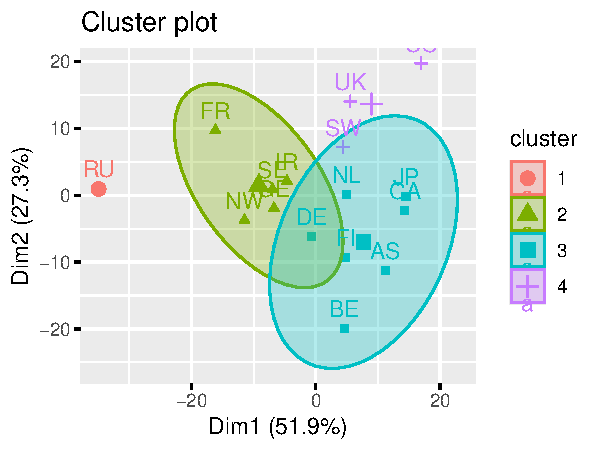
\includegraphics{8_Agrupaciones-041}
\caption{Partición de promedios por país de los indicadores del ARWU }\label{fig:gruposUnisarwu}
\end{figure}
\end{frame}
%
\section{Agrupación jerárquica a partir componentes principales}
\begin{frame}{Agrupación jerárquica a partir de componentes principales}
{Algoritmo}
\begin{itemize}
\item Realizar un método factorial a los datos originales con lo cual se reduce la dimensionalidad y se identifican los factores que se utilizarán para el agrupamiento.
\item Seleccionar $q \le p$ factores para usarlos como información de arranque para la  agrupación
\item Tipificar las grupos comparando las estadísticas básicas de las variables originales por grupos con las mísmas estadísticas pero calculadas para el conjunto completo de datos.
\item Posicionar las grupos en los planos factoriales.
\end{itemize}
\end{frame}
%
\begin{frame}[fragile]
{Ejemplo Arwu 2}
{Agrupamiento de paises por puntajes promedio de los indicadores del ARWU a partir de un ACP.}
\begin{block}{ARWU}
\begin{table}[!h]
\centering
\caption{\label{tab:vp_sue}Valores propios y varianzas del ACP de indicadores del SUE}
\centering
\resizebox{\ifdim\width>\linewidth\linewidth\else\width\fi}{!}{
\begin{tabular}[t]{lrrr}
\toprule
  & eigenvalue & percentage of variance & cumulative percentage of variance\\
\midrule
\cellcolor{gray!10}{comp 1} & \cellcolor{gray!10}{2.57} & \cellcolor{gray!10}{42.75} & \cellcolor{gray!10}{42.75}\\
comp 2 & 1.60 & 26.66 & 69.41\\
\cellcolor{gray!10}{comp 3} & \cellcolor{gray!10}{0.73} & \cellcolor{gray!10}{12.19} & \cellcolor{gray!10}{81.60}\\
comp 4 & 0.71 & 11.82 & 93.42\\
\cellcolor{gray!10}{comp 5} & \cellcolor{gray!10}{0.33} & \cellcolor{gray!10}{5.49} & \cellcolor{gray!10}{98.91}\\
\addlinespace
comp 6 & 0.07 & 1.09 & 100.00\\
\bottomrule
\end{tabular}}
\end{table}
\end{block}
\end{frame}
%
\begin{frame}[fragile]
{Ejemplo Arwu 2}
{Agrupamiento de paises por puntajes promedio de los indicadores del ARWU a partir de un ACP.}
\begin{block}{ARWU}
\begin{table}[!h]
\centering
\caption{\label{tab:coor}Coordenadas sobre los primeros cuatro factores del ACP de indicadores del SUE}
\centering
\begin{tabular}[t]{lrrrr}
\toprule
  & Dim.1 & Dim.2 & Dim.3 & Dim.4\\
\midrule
\cellcolor{gray!10}{HiCi} & \cellcolor{gray!10}{0.7940681} & \cellcolor{gray!10}{0.4657882} & \cellcolor{gray!10}{0.0767951} & \cellcolor{gray!10}{-0.3426638}\\
PUB & 0.6861647 & -0.0943919 & 0.3739958 & 0.5774505\\
\cellcolor{gray!10}{N.S} & \cellcolor{gray!10}{0.6773997} & \cellcolor{gray!10}{0.7013240} & \cellcolor{gray!10}{0.0762402} & \cellcolor{gray!10}{-0.0739793}\\
PCP & -0.2382619 & 0.6933177 & -0.5263108 & 0.4275308\\
\cellcolor{gray!10}{Alumni} & \cellcolor{gray!10}{-0.6725637} & \cellcolor{gray!10}{0.4023454} & \cellcolor{gray!10}{0.5033715} & \cellcolor{gray!10}{0.1706912}\\
\addlinespace
Award & -0.7041037 & 0.4891066 & 0.2216985 & -0.2025993\\
\bottomrule
\end{tabular}
\end{table}\end{block}
\end{frame}
% 
\begin{frame}[fragile]
{Ejemplo Arwu 2}
{Agrupamiento de paises por puntajes promedio de los indicadores del ARWU a partir de un ACP.}
\begin{block}{ARWU}
\begin{table}[!h]
\centering
\caption{\label{tab:contr}Contribuciones a la varianza de los primeros cuatro factores del ACP de indicadores del SUE}
\centering
\begin{tabular}[t]{lrrrr}
\toprule
  & Dim.1 & Dim.2 & Dim.3 & Dim.4\\
\midrule
\cellcolor{gray!10}{HiCi} & \cellcolor{gray!10}{24.581571} & \cellcolor{gray!10}{13.5639819} & \cellcolor{gray!10}{0.8066381} & \cellcolor{gray!10}{16.5540208}\\
Award & 19.327132 & 14.9560637 & 6.7226040 & 5.7868555\\
\cellcolor{gray!10}{PUB} & \cellcolor{gray!10}{18.354852} & \cellcolor{gray!10}{0.5570311} & \cellcolor{gray!10}{19.1313383} & \cellcolor{gray!10}{47.0106674}\\
N.S & 17.888922 & 30.7501777 & 0.7950239 & 0.7715921\\
\cellcolor{gray!10}{Alumni} & \cellcolor{gray!10}{17.634412} & \cellcolor{gray!10}{10.1206471} & \cellcolor{gray!10}{34.6568522} & \cellcolor{gray!10}{4.1076114}\\
\addlinespace
PCP & 2.213111 & 30.0520985 & 37.8875435 & 25.7692528\\
\bottomrule
\end{tabular}
\end{table}\end{block}
\end{frame}
% 
\begin{frame}[fragile]
{Ejemplo Arwu 2}
{Agrupamiento de paises por puntajes promedio de los indicadores del ARWU a partir de un ACP.}
\begin{block}{ARWU}
\begin{table}[!h]
\centering
\caption{\label{tab:cos2}Cosenos cuadrados sobre los primeros cuatro factores del ACP de indicadores del SUE}
\centering
\begin{tabular}[t]{lrrrr}
\toprule
  & Dim.1 & Dim.2 & Dim.3 & Dim.4\\
\midrule
\cellcolor{gray!10}{HiCi} & \cellcolor{gray!10}{0.6305441} & \cellcolor{gray!10}{0.2169586} & \cellcolor{gray!10}{0.0058975} & \cellcolor{gray!10}{0.1174185}\\
Award & 0.4957620 & 0.2392253 & 0.0491502 & 0.0410465\\
\cellcolor{gray!10}{PUB} & \cellcolor{gray!10}{0.4708220} & \cellcolor{gray!10}{0.0089098} & \cellcolor{gray!10}{0.1398729} & \cellcolor{gray!10}{0.3334490}\\
N.S & 0.4588704 & 0.4918553 & 0.0058126 & 0.0054729\\
\cellcolor{gray!10}{Alumni} & \cellcolor{gray!10}{0.4523419} & \cellcolor{gray!10}{0.1618818} & \cellcolor{gray!10}{0.2533829} & \cellcolor{gray!10}{0.0291355}\\
\addlinespace
PCP & 0.0567687 & 0.4806894 & 0.2770031 & 0.1827826\\
\bottomrule
\end{tabular}
\end{table}\end{block}
\end{frame}
% 
\begin{frame}[fragile]
Para utilizar solamente los dos primeros factores es necesario correr de nuevo el PCA para retener solo éstos dos.
\begin{Schunk}
\begin{Sinput}
> res.PCA2<-PCA(mediaspais, ncp = 2) 
\end{Sinput}
\end{Schunk}
Entonces se utiliza la salida del PCA con estas dos primeras componentes:
\begin{Schunk}
\begin{Sinput}
> res.hcpc<-HCPC(res.PCA2, 
+                nb.clust = -1, min = 3, max = 6, , proba=0.1)
\end{Sinput}
\end{Schunk}
\end{frame}
%
\begin{frame}[fragile]
\begin{figure}[H]
\centering
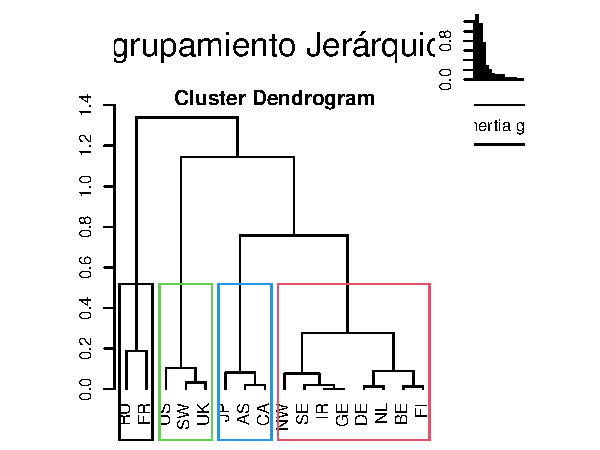
\includegraphics{8_Agrupaciones-clusterPCA4_12}
\caption{El dendrograma sugiere cuatro grupos uno de los cuales está formado por Rusia y Francia, los dos países que sobresalen en el plano de países}\label{fig:dendropaises4grupos2}
\end{figure}
\end{frame}
%
\begin{frame}[fragile]
{Tipificación de los grupos}
\begin{block}{Datos originales y pertenencia a los grupos}
\begin{table}[!h]
\centering
\resizebox{\ifdim\width>\linewidth\linewidth\else\width\fi}{!}{
\begin{tabular}{lrrrrrrl}
\toprule
  & Alumni & Award & HiCi & N.S & PUB & PCP & clust\\
\midrule
\cellcolor{gray!10}{FR} & \cellcolor{gray!10}{39.10000} & \cellcolor{gray!10}{31.30000} & \cellcolor{gray!10}{16.63333} & \cellcolor{gray!10}{22.76667} & \cellcolor{gray!10}{45.90000} & \cellcolor{gray!10}{34.06667} & \cellcolor{gray!10}{1}\\
RU & 46.80000 & 34.10000 & 0.00000 & 9.60000 & 52.40000 & 31.20000 & 1\\
\cellcolor{gray!10}{BE} & \cellcolor{gray!10}{7.50000} & \cellcolor{gray!10}{15.40000} & \cellcolor{gray!10}{17.60000} & \cellcolor{gray!10}{15.10000} & \cellcolor{gray!10}{54.40000} & \cellcolor{gray!10}{30.40000} & \cellcolor{gray!10}{2}\\
DE & 19.60000 & 21.50000 & 16.60000 & 24.75000 & 52.40000 & 28.85000 & 2\\
\cellcolor{gray!10}{FI} & \cellcolor{gray!10}{16.00000} & \cellcolor{gray!10}{17.80000} & \cellcolor{gray!10}{22.80000} & \cellcolor{gray!10}{20.60000} & \cellcolor{gray!10}{52.70000} & \cellcolor{gray!10}{28.20000} & \cellcolor{gray!10}{2}\\
\addlinespace
GE & 27.48000 & 22.62000 & 17.48000 & 21.86000 & 46.96000 & 27.42000 & 2\\
\cellcolor{gray!10}{IR} & \cellcolor{gray!10}{31.50000} & \cellcolor{gray!10}{19.90000} & \cellcolor{gray!10}{24.90000} & \cellcolor{gray!10}{20.80000} & \cellcolor{gray!10}{41.60000} & \cellcolor{gray!10}{26.50000} & \cellcolor{gray!10}{2}\\
NL & 23.70000 & 18.15000 & 27.90000 & 25.15000 & 48.00000 & 29.25000 & 2\\
\cellcolor{gray!10}{NW} & \cellcolor{gray!10}{22.00000} & \cellcolor{gray!10}{33.30000} & \cellcolor{gray!10}{17.60000} & \cellcolor{gray!10}{13.50000} & \cellcolor{gray!10}{46.60000} & \cellcolor{gray!10}{24.30000} & \cellcolor{gray!10}{2}\\
SE & 24.36667 & 29.60000 & 20.63333 & 20.26667 & 45.63333 & 29.63333 & 2\\
\addlinespace
\cellcolor{gray!10}{SW} & \cellcolor{gray!10}{22.26667} & \cellcolor{gray!10}{26.60000} & \cellcolor{gray!10}{28.50000} & \cellcolor{gray!10}{30.56667} & \cellcolor{gray!10}{46.80000} & \cellcolor{gray!10}{36.20000} & \cellcolor{gray!10}{3}\\
UK & 28.66364 & 30.97273 & 33.10000 & 31.56364 & 55.47273 & 29.10000 & 3\\
\cellcolor{gray!10}{US} & \cellcolor{gray!10}{25.65556} & \cellcolor{gray!10}{29.60926} & \cellcolor{gray!10}{44.42407} & \cellcolor{gray!10}{37.37037} & \cellcolor{gray!10}{55.42963} & \cellcolor{gray!10}{30.79074} & \cellcolor{gray!10}{3}\\
AS & 17.30000 & 8.90000 & 26.40000 & 21.63333 & 56.10000 & 27.73333 & 4\\
\cellcolor{gray!10}{CA} & \cellcolor{gray!10}{21.67500} & \cellcolor{gray!10}{14.25000} & \cellcolor{gray!10}{31.50000} & \cellcolor{gray!10}{26.70000} & \cellcolor{gray!10}{63.22500} & \cellcolor{gray!10}{24.92500} & \cellcolor{gray!10}{4}\\
\addlinespace
JP & 23.62000 & 12.58000 & 28.94000 & 32.20000 & 63.32000 & 29.36000 & 4\\
\bottomrule
\end{tabular}}
\end{table}\end{block}
\end{frame}
%
%
\begin{frame}[fragile]
{Descripción de los grupos por las variables}
\begin{table}[!h]
\centering\caption{\label{tab:grps1}Grupo 1: FR, RU}

\centering
\resizebox{\ifdim\width>\linewidth\linewidth\else\width\fi}{!}{
\begin{tabular}[t]{lrrrrrr}
\toprule
  & v.test & Mean in category & Overall mean & sd in category & Overall sd & p.value\\
\midrule
\cellcolor{gray!10}{Alumni} & \cellcolor{gray!10}{3.009886} & \cellcolor{gray!10}{42.950000} & \cellcolor{gray!10}{24.82672} & \cellcolor{gray!10}{3.850000} & \cellcolor{gray!10}{8.814208} & \cellcolor{gray!10}{0.0026135}\\
Award & 1.844021 & 32.700000 & 22.91137 & 1.400000 & 7.770565 & 0.0651801\\
\cellcolor{gray!10}{PCP} & \cellcolor{gray!10}{1.695601} & \cellcolor{gray!10}{32.633333} & \cellcolor{gray!10}{29.24557} & \cellcolor{gray!10}{1.433333} & \cellcolor{gray!10}{2.924735} & \cellcolor{gray!10}{0.0899616}\\
HiCi & -2.333446 & 8.316667 & 23.43817 & 8.316667 & 9.486235 & 0.0196248\\
\bottomrule
\end{tabular}}
\end{table}\begin{table}[!h]
\centering\caption{\label{tab:grps1}Grupo 2: BE, FI, GE, IR, NL, NW SE}

\centering
\resizebox{\ifdim\width>\linewidth\linewidth\else\width\fi}{!}{
\begin{tabular}[t]{lrrrrrr}
\toprule
  & v.test & Mean in category & Overall mean & sd in category & Overall sd & p.value\\
\midrule
\cellcolor{gray!10}{N.S} & \cellcolor{gray!10}{-1.730892} & \cellcolor{gray!10}{20.25333} & \cellcolor{gray!10}{23.40171} & \cellcolor{gray!10}{3.862679} & \cellcolor{gray!10}{7.044696} & \cellcolor{gray!10}{0.0834711}\\
PUB & -2.018794 & 48.53667 & 51.68379 & 4.026609 & 6.037650 & 0.0435087\\
\bottomrule
\end{tabular}}
\end{table}
\end{frame}

\begin{frame}[fragile]
{Descripción de los grupos por las variables}
\begin{table}[!h]
\centering\caption{\label{tab:grps1}Grupo 3: SW, UK, USA}

\centering
\resizebox{\ifdim\width>\linewidth\linewidth\else\width\fi}{!}{
\begin{tabular}[t]{lrrrrrr}
\toprule
  & v.test & Mean in category & Overall mean & sd in category & Overall sd & p.value\\
\midrule
\cellcolor{gray!10}{N.S} & \cellcolor{gray!10}{2.579008} & \cellcolor{gray!10}{33.16689} & \cellcolor{gray!10}{23.40171} & \cellcolor{gray!10}{3.000046} & \cellcolor{gray!10}{7.044696} & \cellcolor{gray!10}{0.0099085}\\
HiCi & 2.334554 & 35.34136 & 23.43817 & 6.691377 & 9.486235 & 0.0195667\\
\cellcolor{gray!10}{PCP} & \cellcolor{gray!10}{1.771427} & \cellcolor{gray!10}{32.03025} & \cellcolor{gray!10}{29.24557} & \cellcolor{gray!10}{3.028177} & \cellcolor{gray!10}{2.924735} & \cellcolor{gray!10}{0.0764897}\\
\bottomrule
\end{tabular}}
\end{table}\begin{table}[!h]
\centering\caption{\label{tab:grps1}Grupo 4: JP, AS, CA}

\centering
\resizebox{\ifdim\width>\linewidth\linewidth\else\width\fi}{!}{
\begin{tabular}[t]{lrrrrrr}
\toprule
  & v.test & Mean in category & Overall mean & sd in category & Overall sd & p.value\\
\midrule
\cellcolor{gray!10}{PUB} & \cellcolor{gray!10}{2.834354} & \cellcolor{gray!10}{60.88167} & \cellcolor{gray!10}{51.68379} & \cellcolor{gray!10}{3.381371} & \cellcolor{gray!10}{6.037650} & \cellcolor{gray!10}{0.0045918}\\
Award & -2.634080 & 11.91000 & 22.91137 & 2.234920 & 7.770565 & 0.0084366\\
\bottomrule
\end{tabular}}
\end{table}% 
\end{frame}
%

\begin{frame}
\setkeys{Gin}{width=1\textwidth, height=0.8\textheight,keepaspectratio} % para redefinir el tama?o de los graficos
\begin{figure}[H]
	\centering
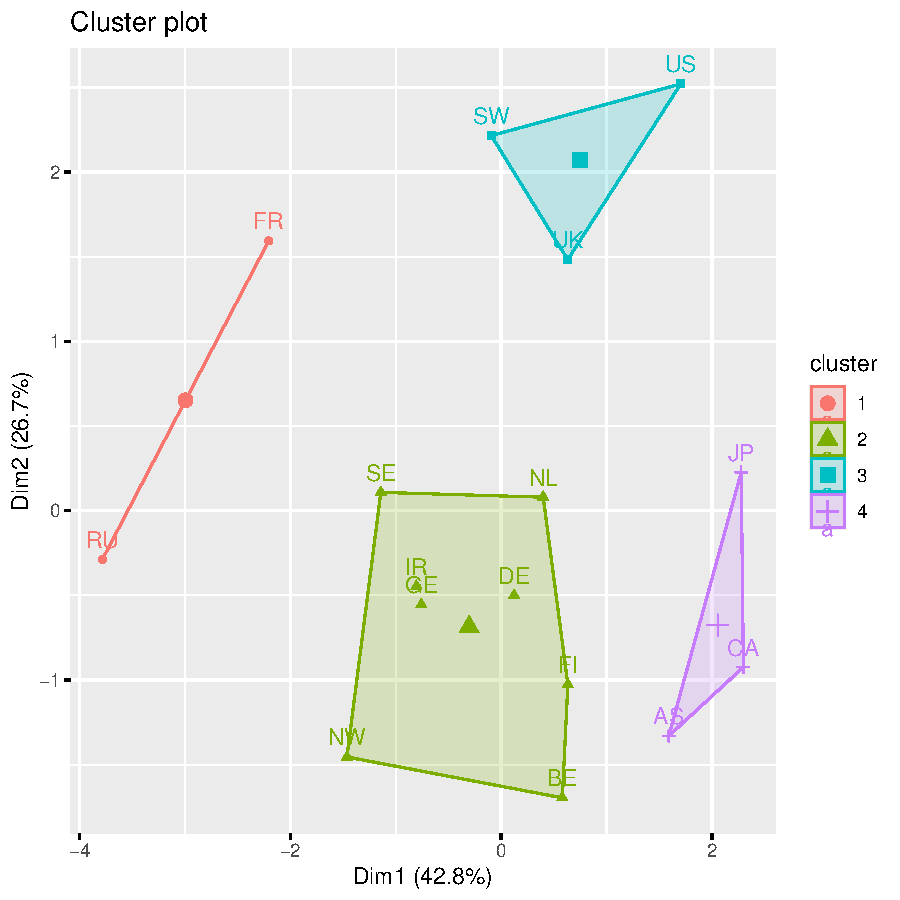
\includegraphics{8_Agrupaciones-052}
	\caption{Proyección de los grupos sobre el plano 1-2}\label{fig:gruposARWU}
\end{figure}
\end{frame}
%
\begin{frame}
\setkeys{Gin}{width=1\textwidth, height=0.8\textheight,keepaspectratio} % para redefinir el tama?o de los graficos
\begin{figure}[H]
	\centering
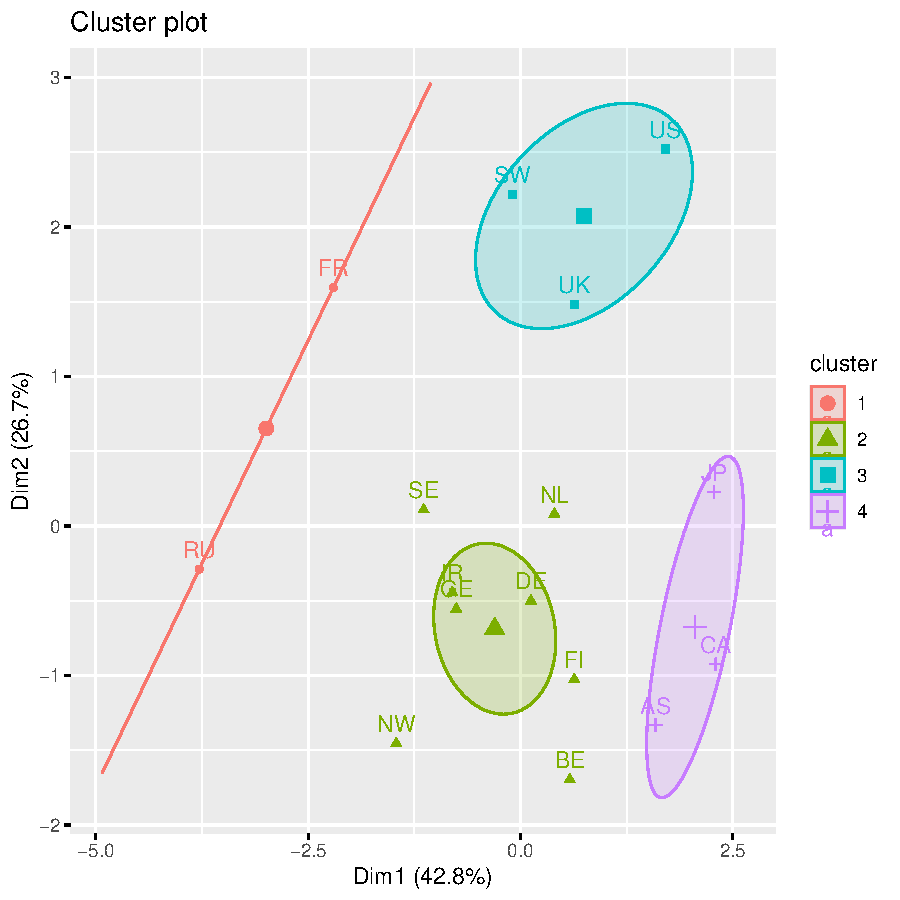
\includegraphics{8_Agrupaciones-053}
	\caption{Proyección de los grupos sobre el plano 1-2}\label{fig:gruposARWU}
\end{figure}
\end{frame}
% \begin{frame}
% 
% \end{frame}
%
% \begin{frame}
% 
% \end{frame}
%
% \begin{frame}
% 
% \end{frame}
%
% \begin{frame}
% 
% \end{frame}
\begin{frame}{Referencias bibliográficas}
\bibliography{BiblioMultivariado}
\end{frame}
% 
\end{document}


